\documentclass[12pt]{report}

%  ********** Incluir packages **********
\usepackage[english,spanish]{babel} % Out: Idiomas usados
\usepackage{lmodern}           % Out: Fuente "Latin Modern"
\usepackage[T1]{fontenc}       % Out: Encoding de la fuente
\usepackage[utf8]{inputenc}    % In:  Encoding de los archivos de entrada
\usepackage{graphicx}          % Importar imágenes y gráficos
\usepackage{datetime}          % Acceso a variables de fecha
\usepackage{fancyhdr}          % Cabecera de página (numeración)
\usepackage{titlesec}          % Cambiar formato de título en los capitulos y otros.
\usepackage[table]{xcolor}     % Colores
\usepackage{dcolumn}           % Columnas alineadas por punto decimal
%\usepackage{listings}          % Código fuente
%\usepackage{array}             %
\usepackage{caption}           % Soporte para subfiguras
\usepackage{subcaption}        % Soporte para subfiguras
\usepackage{amsfonts}          %
\usepackage{mathtools}         %
\usepackage{enumitem}          % Insertar símbolos en Item
\usepackage[hyperref=true]{acro} % Acrónimos
\usepackage[bookmarks=true,bookmarksnumbered, colorlinks=t, hidelinks, breaklinks]{hyperref}
% Margenes y tamaño de la página
\usepackage[letterpaper, top=2.5cm, bottom=2cm, left=2.5cm, right=2cm, headsep=0.3cm]{geometry}

%  ********** Definir autor, prof. patrocinante, título y fecha de la memoria **********
\newcommand{\AuthorName}{Aldo Nicolás Mellado Opazo}
\newcommand{\AdvisorNameA}{Dr. Sergio Sobarzo Guzmán.}
\newcommand{\MainTitle}{Sistema de posicionamiento indoor mediante seguimiento de direcciones MAC de equipos móviles}
\newcommand{\Career}{Ingeniería Civil en Telecomunicaciones}
\newcommand{\CTitle}{Ingeniero Civil en Telecomunicaciones}
%\newcommand{\MyCustomDate}{Julio de 2015} % Comentar para poner fecha automáticamente

%  ********** Configurar packages y otras cosas **********
% -- Bibliography style (BibTeX) --
\bibliographystyle{IEEEtran}
% -- graphicx --
\graphicspath{{./images/}}
%
% -- fancyhdr (numaración de páginas) --
\fancypagestyle{plain}{%
\fancyhf{}
\fancyhead[R]{\thepage}
\renewcommand{\headrulewidth}{0pt}
\renewcommand{\footrulewidth}{0pt}
}
%
% -- titlesec (estilo de título) --
\titleformat{\chapter}[hang]{\bfseries\huge}{\thechapter.}{2ex}{}
\titlespacing{\chapter}{0cm}{0cm}{0cm}
%
% -- caption y subcaption --
\captionsetup[figure]{skip=2pt}
\captionsetup[subfigure]{skip=0pt}
\captionsetup[table]{skip=2pt}
% -- acro: Acrónimos --
% Para arónimos en inglés
\newcommand{\MyCustomListStyle}[1]{(del inglés \itshape{#1})}
\acsetup{ foreign-format = {del inglés \itshape} }
\acsetup{ list-foreign-format = {\MyCustomListStyle} }

% ********** Interlineado, salto de párrafo y sangría **********
% Para interlineado de 1.5  poner: 1.3
% Para interlineado de 2.0 poner: 1.6
\linespread{1.3}
%\setlength{\parindent}{1cm}
\setlength{\parskip}{0.4cm}


% Archivo con definición de acrónimos

% Template: \DeclareAcronym{} { short = , long = , foreign = }
\DeclareAcronym{ASIC}  { short = ASIC, long = circuito integrado de aplicación específica, foreign = Application-Specific Integrated Circuit}
\DeclareAcronym{CMOS}  { short = CMOS, long = semiconductor complementario de óxido metálico, foreign = Complementary Metal Oxide Semiconductor}
\DeclareAcronym{FPGA}  { short = FPGA, long = arreglo de compuertas programables, foreign = Field Programmable Gate Array}
\DeclareAcronym{NAVSAT}{short= NAVSAT, long= Sistema Satelital de Navegación Naval, foreign= Navy Navigation Satellite System}
\DeclareAcronym{GPS}{short = GPS,long = Sistema de Posicionamiento Global, foreign = Global Positioning System}
\DeclareAcronym{AP}{short = AP,long  = Punto de Acceso, foreign= Access Point}
\DeclareAcronym{MAC}{short= MAC,long = Control de Acceso al Medio, foreign =Media Access Control}
\DeclareAcronym{RNN}{short= RNN,long = Red Neuronal Recurrente, foreign = Recurrent Neural Network}
\DeclareAcronym{IPS}{short = IPS,long  = Sistema de Posicionamiento en Interiores, foreign= Indoor Positioning System}
\DeclareAcronym{RSSI}{short= RSSI, long = Indicador de Intensidad de Señal Recibida, foreign = Received Signal Strengh Indicator}
\DeclareAcronym{AoA}{short= AoA,long= Ángulo de llegada ,foreign = Angle of Arrival}
\DeclareAcronym{ToA}{short= ToA,long= Tiempo de llegada ,foreign = Time of Arrival}
\DeclareAcronym{ToF}{short= ToF,long = Tiempo de Vuelo ,foreign = Time of Flight}
\DeclareAcronym{KNN}{short= KNN ,long = K-Vecinos más Cercanos, foreign= K-Nearest Neighbour}
\DeclareAcronym{RSS}{short = RSS, long= Nivel de Intensidad de Señal Recibida, foreign = Received Signal Strenght}
\DeclareAcronym{TDoA}{short = TDoA, long = Diferencia de Tiempo de Llegada, foreign = Time Difference of Arrival}
\DeclareAcronym{RToF}{short=  RToF, long= Ruta de Viaje de Vuelo, foreign = Round-Trip Time of Flight}
\DeclareAcronym{NLOS}{short = NLOS, long = No Línea de Vista, foreign = None Line of Sight}
\DeclareAcronym{RN}{short = RN, long = Redes Neuronales, foreign = Artificial Neural Network}
\DeclareAcronym{RN  N}{short = RNN, long = Red Neuronal Recurrente, foreign = Recurrent Neural Network}
\DeclareAcronym{KWNN}{short=KWNN, long= K-Vecino Ponderado Más Cercano,foreign = K-Weighted nearest neighbor}
\DeclareAcronym{SVM}{short = SVP,long = Máquinas de vectores de soporte,foreign = Support Vector Machine }
\DeclareAcronym{SMP}{short = SMP,long = Polígono más pequeño de M-Vértices ,foreign = Smallest M-Vertex Polygon}
\DeclareAcronym{LOS}{short = LOS,long = Línea de Vista, foreign = Line of Sight}
\DeclareAcronym{FCC}{short = FCC, long = Comisión Federal de Comunicaciones, foreign = Federal Communications Commission}
\DeclareAcronym{RTT}{short=RTT,long = Tiempo-de-Viaje, foreign = Round-Trip-Time}
\DeclareAcronym{BLE}{short=BLE, long = Bluetooth de Baja Energía, foreign = Bluetooth Low Energy}
\DeclareAcronym{UWB}{short = UWB, long = Banda Ultra Ancha, foreign = Ultra Wide-Band}

\begin{document}
% ******************** Algunas definiciones ********************
\renewcommand{\contentsname}{Índice General}
\renewcommand{\listfigurename}{Índice de Figuras}
\renewcommand{\listtablename}{Índice de Tablas}
\renewcommand{\figurename}{\textbf{Fig.}}
\renewcommand{\tablename}{\textbf{Tabla}}


% ******************** Portada ********************
	% Hoja 1
	\pdfbookmark{Portada}{portada}
	\thispagestyle{empty}
	\begin{titlepage}
\begingroup

% Esta página usa interlineado simple sin saltos de párrafo
\linespread{1}\selectfont
\setlength{\parskip}{0pt}
	
{ \vspace*{2 pc} }

\begin{center}
	\textbf{\LARGE UNIVERSIDAD DE CONCEPCIÓN} \\[0.4 pc]
	{\large FACULTAD DE INGENIERÍA} \\[0.4 pc]
	{ DEPARTAMENTO DE INGENIERÍA ELÉCTRICA} \\[0.4 pc]
\end{center}

\vspace{6 pc}

\noindent\begin{minipage}{0.35\textwidth}\hfill\end{minipage}
%
\begin{minipage}[t]{0.25\textwidth}
	\centering
	
\includegraphics[width=3.2cm]{logos/logo_udec}
\end{minipage}
%
\hspace*{0.5cm}
%
\begin{minipage}{0.34\textwidth}
	Profesor Patrocinante: \\[0.4 pc] \textbf{\AdvisorNameA} \\
	\vskip 4.3cm
	Informe de Memoria de Título \\
	para optar al título de: \\[0.4 pc]
	\textbf{Ingeniero Civil en Telecomunicaciones}
\end{minipage}

\vspace{9 pc}

\begin{center}
	\textbf{\LARGE \MainTitle}
\end{center}
%
%
\vfill
Concepción,
\ifdefined\MyCustomDate
	\MyCustomDate
\else
	{\monthname} de \the\year
\fi
\hfill \AuthorName
%
%
\endgroup
\end{titlepage}


	% Hoja 2
	\thispagestyle{empty}
	\begin{titlepage}
\begingroup

% Esta página usa interlineado simple sin saltos de párrafo
\linespread{1}\selectfont
\setlength{\parskip}{0pt}

% Universidad y supervisor
\begin{minipage}{0.45\textwidth}
	Universidad de Concepción \\ Facultad de Ingeniería \\ Departamento de Ingeniería Eléctrica
\end{minipage}
%
\hfill
%
\begin{minipage}{0.45\textwidth}
	\raggedleft
	Profesor Patrocinante: \\ \AdvisorNameA 
\end{minipage}
%
%
\begin{center} 
	\vspace{5cm}
	
	\textsc{\huge \MainTitle}\\[5.5cm]

	{\large \AuthorName}\\[1.5cm]

	Informe de Memoria de Título\\
	para optar al Título de\\[1.5cm] 

	\CTitle
	\vfill

	% Final de la página
	\ifdefined\MyCustomDate
		{\large \MyCustomDate}
	\else
		{\large {\monthname} \the\year}
	\fi
\end{center}

\endgroup
\end{titlepage}



% ******************** Resumen y agradecimientos ********************
	% Numeración: Romana, i.e. I, II, III, etc.
	% página no numerada
	\newpage
	\pagestyle{plain}
	\pagenumbering{roman}
	\setcounter{secnumdepth}{-1}
%    \chapter{Resumen}

Lorem ipsum dolor sit amet, consectetur adipiscing elit, sed do eiusmod tempor incididunt ut labore et dolore magna aliqua. Ut enim ad minim veniam, quis nostrud exercitation ullamco laboris nisi ut aliquip ex ea commodo consequat. Duis aute irure dolor in reprehenderit in voluptate velit esse cillum dolore eu fugiat nulla pariatur. Excepteur sint occaecat cupidatat non proident, sunt in culpa qui officia deserunt mollit anim id est laborum.

Un \ac{FPGA} se puede usar en las etapas de diseño de un \ac{ASIC}.
Aunque los \acp{FPGA} también tienen otros usos.

\acresetall

    
%    %---------- Primera hoja ----------
\vspace*{\fill}

\begin{flushright}
    {\large Gaudeamus igitur iuvenes dum sumus...}\\
    {\large Tempus Fugit...}\\
    %{\large \emph{Gracias por todo}}
\end{flushright}
\vspace*{\fill}


%---------- Segunda hoja ----------
\newpage
\chapter{Agradecimientos}

Lorem ipsum dolor sit amet, consectetur adipiscing elit, sed do eiusmod tempor incididunt ut labore et dolore magna aliqua. Ut enim ad minim veniam, quis nostrud exercitation ullamco laboris nisi ut aliquip ex ea commodo consequat. Duis aute irure dolor in reprehenderit in voluptate velit esse cillum dolore eu fugiat nulla pariatur. Excepteur sint occaecat cupidatat non proident, sunt in culpa qui officia deserunt mollit anim id est laborum.



% ******************** Índice ********************
    \newpage
    \begingroup
    \setlength{\parskip}{0pt}
    % Profundidad de numeración en el índice
    \setcounter{secnumdepth}{3}
    % Profundidad de numeración en el texto
    \setcounter{tocdepth}{3}
    \pdfbookmark{\contentsname}{toc}
    \tableofcontents
	\endgroup


% ******************** Índice de figuras ********************
	\newpage
	\phantomsection
	\addcontentsline{toc}{chapter}{\listfigurename}
	\listoffigures


% ******************** Índice de tablas ********************
    \newpage
    \phantomsection
    \addcontentsline{toc}{chapter}{\listtablename}
    \listoftables


% ******************** Acrónimos ********************
	\newpage
	\printacronyms[name=Siglas]


% ******************** Capítulos ********************
	% Numeración normal, i.e. 1, 2, 3, etc.
    \newpage
    \pagenumbering{arabic}

    \chapter{Introducción}

\section{Antecedentes históricos}
El ser humano, en la década del 60, ante la incipiente necesidad de saber su posición en el planeta desarrolló un sistema de posicionamiento  llamado OMEGA y posteriormente otro llamado TRANSIT o \ac{NAVSAT}, que  fue resultado del trabajo conjunto de la NASA y el departamento de defensa de los Estados Unidos. Años después este acabó siendo reemplazado debido a la falta de precisión que este tenía, y que alcanzaba un error de hasta 250 metros.

Su sucesor apareció en la década del 70 bajo el nombre de \ac{GPS} y su precisión permitía posicionar un objeto con un error de menos de 5 metros. Esto a través del cálculo del tiempo que tarda en llegar la señal al receptor, es decir, el efecto Doppler.

Funciona actualmente con un mínimo de 24 satélites en órbita sobre la tierra cuyas trayectorias sincronizadas le permiten mapear completamente el planeta y entregar posicionamiento casi exacto a dispositivos móviles y vehículos.

Existen desde ya hace décadas intentos por emular lo logrado con el GPS, pero para espacios interiores, estos intentos han recibido el nombre de \ac{IPS}, que conforme a lo que se presentará en capítulos posteriores han logrado obtener resultados de posición con márgenes de error inferiores a los 3 m. 

\section{Definición del problema}
Las condiciones bajo las cuales es posible para la señal propagarse no se cumplen en todos los ambientes. Existen lugares en que a diferencia de lo que sucede en el exterior, donde la señal se refleja haciendo posible la triangulación de la posición, esta se absorbe parcial o completamente y principalmente corresponden a espacios interiores, tales como una bodega, un centro comercial o una oficina, haciendo que posicionarse dentro de estos espacios sea imposible a través del GPS, es por esto que a fin de brindar nuevas experiencias a usuarios a través del posicionamiento dentro de estos espacios se han desarrollado soluciones utilizando la banda de los 2.4 [GHz] que es la utilizada por, entre otros tecnologías, el Wi-Fi. 

Esta ha sido ampliamente estudiada debido a la alta penetración comercial que ha alcanzado precisamente en estos espacios donde el GPS no da cobertura, sin embargo, dentro de los distintos enfoques en que se han abordado los estudios se tiene que la medición de los niveles de potencia radiada desde los \ac{AP}, a través de los cuales se realiza la triangulación de la posición, se ven altamente afectados por la variación del escenario caracterizado. Este tipo de variaciones pueden ser inducidas por la presencia de personas u objetos que reflejen o absorban la señal.

Es por esto que el método a través del cual se de solución al problema del posicionamiento en interiores debe ser un \ac{IPS} capaz de compensar la incidencia de estas variaciones en el indicador de intensidad de señal recibida (RSSI) dentro de la operación del algoritmo y así, estimar correctamente la posición de objetivo deseado identificable a través de su dirección de \ac{MAC}.

\section{Estado del arte}

En cuánto a los enfoques que se han considerado para evaluar la posición de un dispositivo móvil en un espacio interior se han podido desarrollar diversas soluciones que apuntan de una u otra manera a aproximaciones geométricas. A fin de ordenar según la técnica, la documentación consultada, se hará una clasificación y dentro de las categorías, explicará las investigaciones en el área.

%%%%%%%%%%%%%%%%%%%%%%%%%%%%%%%%%%%%%%%%%%%%%%%%%%%%%%%%%%
                \clearpage 
%%%%%%%%%%%%%%%%%%%%%%%%%%%%%%%%%%%%%%%%%%%%%%%%%%%%%%%%%%

Se abordará siguiendo el esquema que está a continuación:
\begin{figure}[h!]
    \centering
    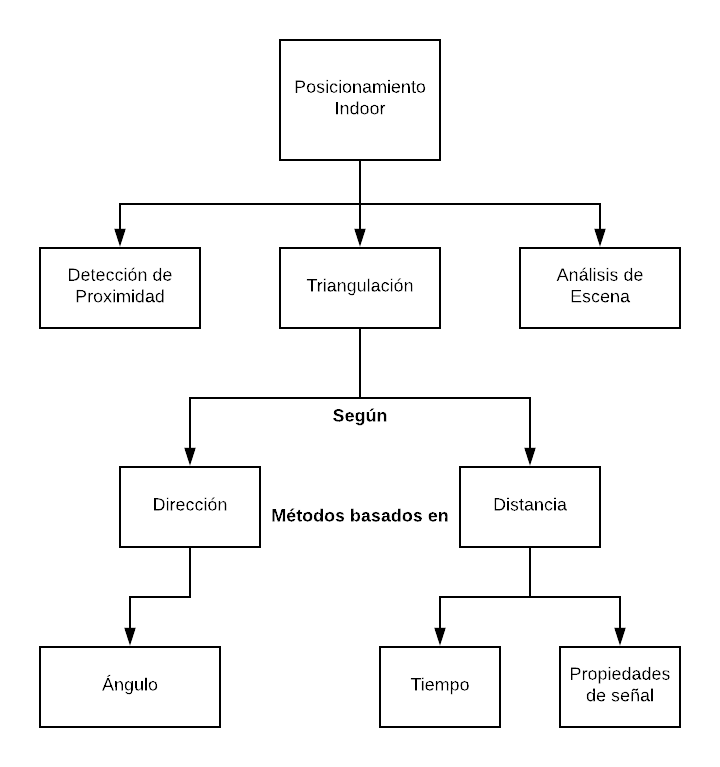
\includegraphics[scale = 0.3]{./images/diagrama}
    \label{fig:diagrama}
\end{figure}

Así, comenzando por el tipo de algoritmos basados en \textit{Detección de proximidad} se tiene que de acuerdo a lo visto en \cite{6}, algunas de las tecnologías que permiten esto, es aquella asociada al uso de beacons; pequeños dispositivos capaces de emitir señales de onda corta por medio de la tecnología Bluetooth, y que puede llegar hasta 50 metros de alcance. Es precisamente en el uso de estos dispositivos que en \cite{20}, los autores, con el fin de integrarlos a tecnologías del IoT, hacen todo un estudio respecto de los distintos tipos de beacons que existen en el mercado, haciendo énfasis en las características asociadas al consumo de energía, al uso del ancho de banda, y de la latencia asociada a la respuesta de los beacons del tipo \ac{BLE}.\\

Presentan además como es que se han integrado estos dispositivos en el comercio, museos, hospitales y estaciones de trabajo, permitiendo así, el surgimiento potencial de una industria interesada en sus bondades. Explican allí que el uso de los beacons se traduce en que cada dispositivo posee una etiqueta única, que para efectos de este trabajo bien puede ser la dirección \ac{MAC}, que al comunicarse con el dispositivo móvil permite a este, enviar una respuesta de cuáles dispositivos tiene a la vista y entonces, comparar el \ac{RSS} para así estimar respecto de cuál beacon está más cercano el usuario.\\

\begin{figure}[h!]
    \centering
    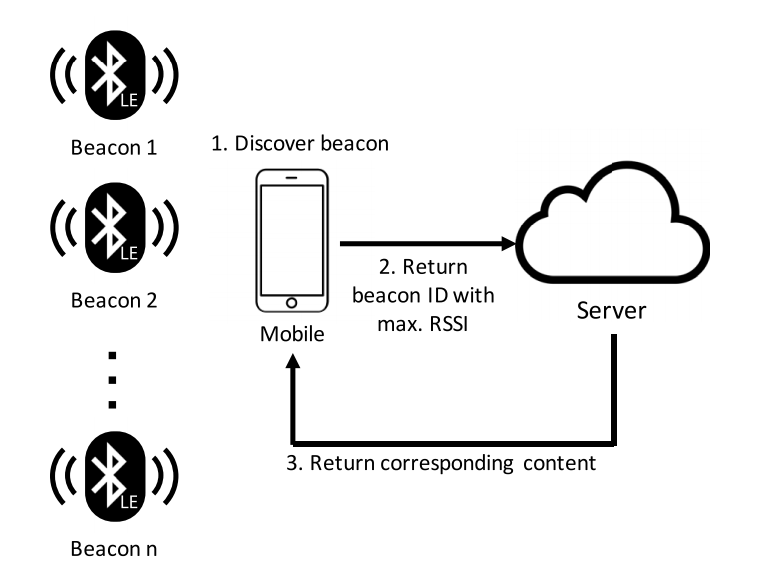
\includegraphics[scale=0.3]{./images/beacon}
    \caption{Imagen de la comparación de la cercanía según el nivel de RSS según un sistema basado en la interacción de beacons BLE}
    \label{fig:my_label}
\end{figure}

Sin embargo, pese a las ventajas asociadas el uso de estos dispositivos, se tiene que así como señalan en \cite{1}, la principal desventaja de algoritmos basados en tecnologías por proximidad, es que generalmente se requiere de hardware adicional, en lugar de los dispositivos que ya se usan e instalan para proveer de internet a usuarios. Además, hay que tener en cuenta que el hardware para este tipo de implementaciones hace uso de una parte no licenciada del espectro, por lo que es altamente susceptible a ser afectada por interferencias de equipos funcionando en la misma banda.\\

Luego, en el tipo de algoritmo basados en \textit{Análisis de Escena} los autores en \cite{1}, presentan un sistema de posicionamiento indoor para navegación que puede funcionar indistintamente si se trata de un smartphone o de una tablet, en tanto se puedan usar los sensores que ya se incluyen en el funcionamiento interno de este. Para el reconocimiento de escena conciben el sistema como uno de dos partes \cite{8}; una offline, que consiste en la extracción de características del entorno y un posterior almacenamiento en una base de datos que servirá para comparar las medidas que se obtengan en la etapa online.Durante esta etapa, la información recolectada es usada par obtener la posición estimada.\\

Las dificultades principales a las que se ven enfrentados estos métodos son los movimientos estructurales a las cuales los espacios se ven sometidos, ya que esto elimina puntos de referencia por simples movimientos de un lugar a otro, lo que conlleva una calibración y medición periódica.\cite{20}\\

Finalmente, en lo que respecta al algoritmo de \textit{Triangulación} se deben hacer algunas subclasificaciones a fin de dejar más claro cómo se ha abordado el problema, de esta manera se tiene que para los métodos basados en:\\
\begin{enumerate}
\item{\textbf{Triangulación:}
    \begin{itemize}
        \item{\textbf{\ac{AoA}}: Referido, como su nombre lo dice, se refiere al ángulo de llegada de la señal del dispositivo móvil, proveniente de una ubicación desconocida, la cual es recibida en múltiples estaciones base. Este algoritmo es evaluado por diversos autores; en \cite{1} los autores lo trabajan como un complemento al uso de los sensores propios del dispositivo, logrando una performance destacable en cuánto a la media del error, sin embargo, no presentan resultados numéricos que permitan conocer el área de cobertura, así como la disponibilidad.\\
            
        En \cite{20}, señalan que una de las desventajas de este método radica en que debido a que no todos los dispositivos están en línea vista con el equipo receptor, la precisión de las mediciones se degrada, haciendo hincapié en que la disposición del arreglo de antenas emisoras juega un rol fundamental en estimar la posición.\\
            
        En \cite{21} comienzan señalando que si bien existen otros algoritmos tales como ToF o TDoF, mucho menos complejos que el de AoA, si es posible implementar un método que alcance una buena precisión pese a las imprecisiones en las mediciones de ángulo y el bajo número de beacons dispuestos. No obstante, en \cite{5} los autores hablan de aproximaciones  híbridos que trabajan con lo mejor de los algoritmos basados en tiempo, y en ángulo para reducir la complejidad que introduce el ambiente indoor. Sin embargo, no logran reducir ni el número de antenas ni el ancho de banda utilizado.}
        \end{itemize}
        }
\item{\textbf{Trilateración}:Este algoritmo puede ser abordado a través de distintas técnicas, algunas de ellas son:
        
    \begin{itemize}
        \item{\textbf{\ac{ToF}}: este concepto está referido a la técnica a través de la cual se realizan cálculos de posición a través del tiempo de llegada de la señal respecto de diversos puntos de referencia.\cite{5}\\
            
        Algunas de las dificultades que exponen los autores en \cite{22} es que la medición de la señal basada en el  tiempo de propagación es que requiere señales de \ac{UWB}, lo que lleva a un consumo de energía considerable, que no ofrece mayor precisión en largas distancias. Muy por el contrario, la precisión de la medición es directamente proporcional a la distancia, pudiendo alcanzar detalle de centímetros cuando la distancia es corta, pero fallas considerables si es que la señal ultrasónica debe viajar sufriendo las atenuaciones del aire así como del efecto multitrayectoria.\\
            
        No obstante, en el sistema \textit{TWINS} de \cite{2} los autores lograron montar un sistema basado en este algoritmo donde utilizan un rango de dos vías, aprovechando el intercambio de tráfico de DATA/ACK, que luego de sortear problemas asociados al protocolo de comunicación, esto es:  ajustar la frecuencia de trabajo, sincronizar los equipos para que funcionen en un mismo tiempo, les permite posicionar usuarios que pueden moverse libremente por el espacio delimitado por el sistema.}\\
        
        \item{\textbf{\ac{RSSI}}: A través de esta técnica los autores en \cite{3} y \cite{4} relacionan los niveles de \ac{RSS} desde los \ac{AP} existentes con la distancia que hay a un AP particular. A través de los modelos de propagación pueden hacer una regresión que, cuando se ha calculado la distancia que hay a los, como mínimo 3, AP se puede entonces crear un sistema de ecuaciones cuyas soluciones son las coordenadas espaciales del objetivo.\\
        
        Otra técnica, algo menos acabada en comparación a lo visto anteriormente, es aquella vista en \cite{13} que hace uso de los niveles de potencia recibida de cada uno de los AP para caracterizar un espacio interior y así, hacer un sistema de coordenadas que permita estimar la posición del usuario. Sin embargo, conocidas las propiedades de los espacios indoor, es sabido que estos son muy dinámicos, que cualquier superficie puede reflejar y absorber potencia, haciendo así variar estos niveles e inducir un margen de error que posicione erróneamente al usuario.\\
        
        Un algoritmo basado en \ac{RSSI}, pero que no usa propiedades geométricas para hacer el posicionamiento es aquell llamado \textit{Fingerprinting Based Indoor Localization}, en \cite{6} los autores lo presentan como una técnica que consiste en dos etapas; la primera, conocida como offline, es la de hacer una colección de los niveles de potencia recibidos en las distintas áreas de interés y almacenarlas en una base de datos que sirva de entrenamiento para las predicciones en las cuales se basará la etapa siguiente; luego, en la etapa \textit{online}, lo que se busca es medir los niveles de potencia y compararlos con el vector de \ac{RSS} que más se le parezca.\\
        
        Para esto, la etapa offline puede verse apoyado por herramientas estadísticas como las de los trabajos \cite{8}, \cite{10},\cite{11},\cite{12} y \cite{14}, o bien, por algoritmos basados técnicas de reconocimiento de patrones probabilísticas y determinísticas tales como KNN, ANN, SVM u otros.\\
        
        \begin{itemize}
            \item {\textbf{\ac{KNN}}: Este algoritmo introducido teóricamente en \cite{7} aparece como un método que autores en \cite{23} usaron KNN para eliminar aquellos puntos individuales en el dataset de muestreo, que bien podría corresponder a aquellos vectores que surgieron de capturar más AP. Luego, usaron SVM para posicionar al usuario. En este trabajo los resultados muestran que el algoritmo híbrido mejora considerablemente la precisión y la velocidad de este.\\
            
            A diferencia de el trabajo anterior, en \cite{24} lo usan para directamente obtener la posición del dispositivo, a la vez que en \cite{25} señalan que el comportamiento de KNN superó en términos de precisión al más sofisticado algoritmo basado en un modelo probabilístico.\\}
            
            \item {\textbf{\ac{RNN}}: \label{RNN} En \cite{15} señalan que las RNN han sido usadas como algoritmos de clasificación en diversas aplicaciones, debido a que puede manejar varias series de datos de tiempo, pero que actualmente no han habido investigaciones que asocien sistemas de posicionamiento indoor al uso de este algoritmo.\\
            
            Por este motivo, ellos desarrollaron un sistema que se basa en RNN y que permite clasificar pares ordenados \textit{(x,y)} basados en el RSSI de cada sensor. Específicamente para implementar un tipo de regresión que permite predecir las coordenadas al considerar cada AP como nodo. Algo parecido a lo que se deseaba conseguir en el trabajo presentado en \cite{28}.\\}
            
            \item {\textbf{\ac{RNA}}: En se \cite{26} aborde el problema de posicionamiento indoor a través del mismo enfoque visto anteriormente en \ref{RNN}, es decir, se busca transformar los RSS a distancias y así determinar las coordenadas del objetivo. La diferencia radica en que acá no se usan AP, sino que otra tecnología llamada ZigBee que también actúa como un sensor de red, señalando que el uso de este, en conjunto con el modelo, trabajan sustancialmente mejor que la técnica de triangulación que por si sola es inestable.\\
            
            Por otro lado en \cite{27} las personas de la investigación comentan que en investigaciones anteriores o en general, en los trabajos que buscan determinar la posición basándose en una ANN utilizan características del ambiente de la \ac{WLAN} para caracterizarlo, estas pueden ser: RSS, que es lo más recurrente a la hora de abordar estos problemas, o bien, \ac{SNR} de los múltiples AP a fin de mapear el espacio en la etapa offline. En contraste a lo anterior señalan que su trabajo es capaz de alcanzar una precisión del 92.86\% solo con el uso de una red de apenas 3 capas que permiten posicionar con una exactitud de tres metros sin incurrir en un margen de error importante, recalcando que si se realiza una división por área, entonces la performance del sistema mejora considerablemente y cuyos resultados fueron contrastados a través de KNN.\\
            
            Finalmente en \cite{28}, al igual que en \cite{27} utilizaron una ANN que se compuso de y capas, y estas a su vez, se desglosaron en 1 capa de entradas, 3 capas ocultas, con 28 nodos cada capa, y 1 de salida, con dos nodos. Interesante señalar que el resultado de agregar 2 capas se tradujo en alcanzar una precisión de 2 metros, que lleva a la conclusión de que la precisión guarda cierta dependencia con el número de nodos y capas ocultas.\\}
        \end{itemize}
        }
    \end{itemize}
        }
\end{enumerate}

%%%%%%%%%%%%%%%%%%%%%%%%%%%%%%%%%%%%%%%%%%%%%%%%%%%%%%%%%%
                \clearpage 
%%%%%%%%%%%%%%%%%%%%%%%%%%%%%%%%%%%%%%%%%%%%%%%%%%%%%%%%%%
\section{Hipótesis de trabajo}
\begin{center}
\textit{''Es posible posicionar un dispositivo, identificable a través de su MAC, en un espacio interior utilizando una Red Neuronal Artificial para compensar las variaciones de RSS de los \ac{AP} usados en la trilateración''}
\end{center}

\section{Objetivos}
A continuación se señalan los objetivos que apuntan a resolver el problema presentado y a probar la hipótesis de trabajo.

\subsection{Objetivo general}
Posicionar un dispositivo móvil, reconocible a través de su \ac{MAC} dentro de un espacio interior, a través de algoritmos de trilateración y \ac{RNA}.

\section{Objetivos específicos}
\begin{itemize}[label={\checkmark}]
\item{Evaluar ventajas y desventajas los modelos utilizados para posicionamiento Indoor}
\item{Realizar mediciones de RSS}
\item{Desarrollar una ANN para hacer el posicionamiento}
\end{itemize}

\section{Alcances y limitaciones}
El alcance de este proyecto estará limitado a encontrar la posición de un dispositivo móvil dentro del espacio del segundo piso de Edificio Tecnológico Mecánico de la Universidad de Concepción. Se ejecutará el algoritmo desarrollado en una laptop personal, utilizando Raspberry Pi como \ac{AP} y el resultado del posicionamiento se desplegará en una interfaz gráfica desarrollada en python.

\section{Metodología}

Para lograr posicionar un dispositivo móvil dentro del espacio interior, se buscará en primera instancia extraer los datos de RSSI obtenidos desde las tarjetas de Red de las placas. Posterior a esto se caracterizará el espacio de trabajo con sus respectivos niveles de RSS. Estas serán usadas para entrenar un modelo que, a través de RNN, pueda detectar la posición en que se halla un usuario, respecto de los niveles de potencia y la certidumbre que arroje el entrenamiento realizado. Finalmente, el resultado será desplegado en una interfaz gráfica.
	\chapter{Marco Teórico}

\section{Introducción}

En este capítulo se sentarán las bases teóricas que soportan y respaldan el trabajar con el algoritmo escogido.

\section{Aplicaciones y aproximaciones en sistemas de posicionamiento indoor}

En cuánto a los sistemas de posicionamiento indoor, diversas documentaciones revisadas señalan la importancia de desarrollar esta tecnología a fin de resolver necesidades ya reconocidas dentro de espacios interiores tales como hospitales, museos, parques, etc. Sin embargo, todos concuerdan en que la tarea no es sencilla y por este motivo se ha intentado abordar este problema de distintas maneras, teniendo cada una sus respectivas ventajas y limitaciones.

La clasificación de estos métodos pasa por si es que en ellos se utilizan propiedades físicas o bien, reconocimiento de imágenes. De este modo, un posible ordenamiento es el que sigue:

\begin{itemize}
    \item{Análisis de escena}
    \item {Detección de proximidad}
    \item{Triangulación}
\end{itemize}

\subsection{Análisis de Escena}
El algoritmo de análisis de escena se refiere al tipo de algoritmo que primero recolecta características de una sala, habitación o espacio y luego estima la posición del objetivo según coincidan los elementos del espacio.

Este algoritmo tiene la ventaja de entregar precisión, a la vez de no requerir la localización de los AP WiFi, y por ende, juega un rol sumamente relevante dentro del algoritmo de posicionamiento indoor. Sin embargo, las desventajas de estos radica en que, computacionalmente hablando, son altamente costosos y que en realidad, no están orientados a entregar posición, sino a reconocer patrones u objetivos, lo que lleva a no conocer coordenadas y geolocalización.

\subsection{Detección de proximidad}\label{Detección de Proximidad}
Este algoritmo es relativamente simple, pero no preciso. Es, en general, utilizado para apoyar el posicionamiento outdoor, ya que este ayuda a estimar la posición de un objetivo utilizando la relación de proximidad entre un objetivo y los Puntos de Acceso cercanos. Cuando el dispositivo móvil objetivo recibe diferentes señales de los distintos AP, permite asociar la intensidad de señal más fuerte a una ubicación particular. 

La precisión de este algoritmo viene dada por la distribución de densidad y el rango de señal de los AP, de modo que si utilizamos antenas adicionales, podemos mejorar la confiabilidad de los resultados, no obstante, esto podría encarecer la implementación.

\subsection{Triangulación}
Este método utiliza propiedades geométricas de triángulos para determinar la ubicación. Tiene dos derivaciones, angulación y lateración. De la primera, se desprende la  técnica de angulación que se basa en la fase de la señal (AoA), mientras que de la segunda, aquellas basadas en la medida de la propagación por tiempo (ToA, TDOA y RTOF) y en los niveles de intensidad de señal recibida (RSSI). 


\begin{figure}[h!]
    \centering
    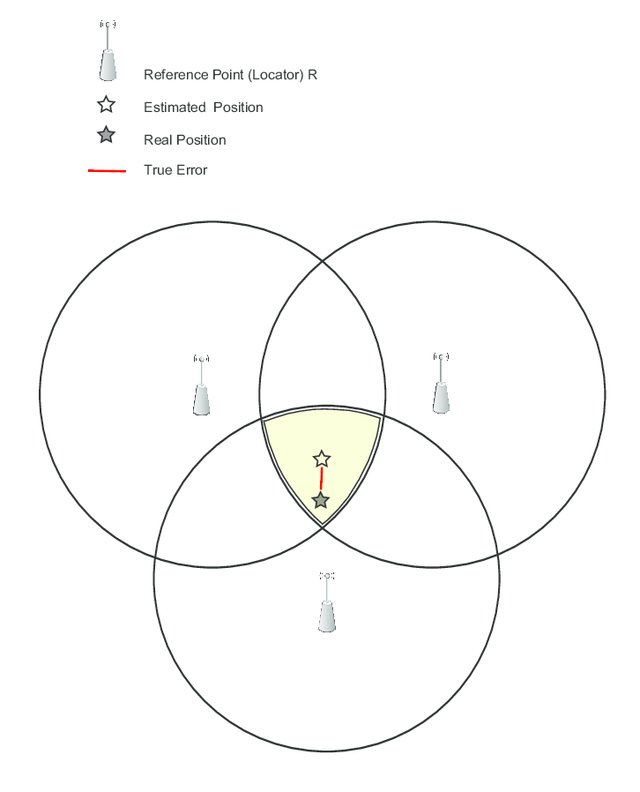
\includegraphics[scale=1]{./images/trilat}
    \caption{Algoritmo de Triangulación}
    \label{fig:Triangulación}
\end{figure}

\subsubsection{\textbf{Angulación}}
    \begin{enumerate}
        \item {\textbf{\ac{AoA}}: es una técnica que determina el ángulo de llegada de la señal, respecto de la ubicación conocida de estaciones base a través de envío de múltiples mensajes desde el Dispositivo móvil hacia el AP. Dado que la precisión de la medición del ángulo de llegada es la que permite estimar la posición, se tiene que estas deben ser altamente direccionales o bien, tratarse de un arreglo de antenas, lo que encarece el costo de sistemas que implementen este tipo de solución. Además, se tiene que esta técnica ve alteradas sus mediciones debido a efectos de la propagación multicamino de la señal cuando se trata de dispositivos que no se hallan en \ac{NLOS}.
        
        \begin{figure}[h!]
            \centering
            \begin{subfigure}[b]{0.3\textwidth}
               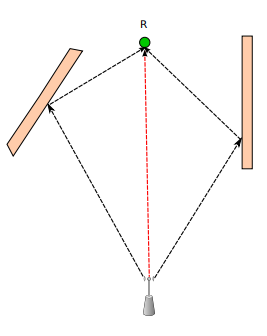
\includegraphics[width=\textwidth]{./images/los}
                \caption{Señal enviada en \ac{LOS}}
                \label{fig:LOS}
            \end{subfigure}
            \begin{subfigure}[b]{0.315\textwidth}
             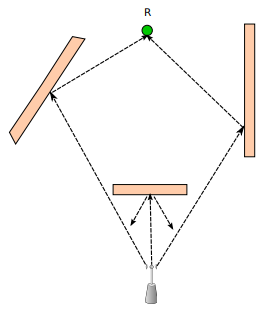
\includegraphics[width=\textwidth]{./images/nlos}
                \caption{Señal enviada en \ac{NLOS}}
                \label{fig:NLOS}
            \end{subfigure}
        \end{figure}
        
%%%%%%%%%%%%%%%%%%%%%%%%%%%%%%%%%%%%%%%%%%%%%%%%%%%%%%%%%%
                \clearpage 
%%%%%%%%%%%%%%%%%%%%%%%%%%%%%%%%%%%%%%%%%%%%%%%%%%%%%%%%%%

        
        Por esta razón, el sistema, aunque preciso en espacios exteriores, no es del todo idóneo para espacios interiores, ya que las reflexiones que se producen en paredes y otros objetos que cambian significativamente la dirección o ángulo de llegada de la señal y por tanto, degradan la precisión de la estimación de posición.
        
        \begin{figure}[h!]
            \centering
            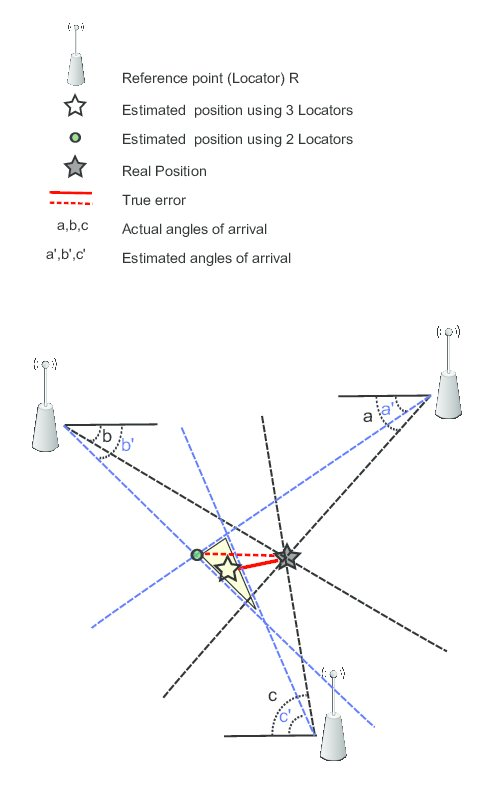
\includegraphics[scale=1.2]{./images/aoa}
            \caption{Técnica de Ángulo de Llegada (AoA)}
            \label{fig:AoA}
        \end{figure}
        }
    \end{enumerate}

%%%%%%%%%%%%%%%%%%%%%%%%%%%%%%%%%%%%%%%%%%%%%%%%%%%%%%%%%%
                \clearpage 
%%%%%%%%%%%%%%%%%%%%%%%%%%%%%%%%%%%%%%%%%%%%%%%%%%%%%%%%%%

\subsubsection{\textbf{Lateración}}

\begin{itemize}
    \item{\textbf{Técnicas basadas en la propagación por tiempo}
    
    \begin{enumerate}
        \item {\textbf{\ac{ToA}}: \label{ToA} El tiempo de llegada aparece como el tiempo de viaje del transmisor hasta el receptor y permite, si es que se le multiplica por la velocidad de la luz, obtener la distancia que separa ambos dispositivos. Para medir el tiempo de llegada en el aire, este método requiere sincronización previa de los dispositivos, que para hacer posicionamiento en el espacio, requiere de al menos 4 transmisores.
        
         \begin{figure}[h!]
            \centering
            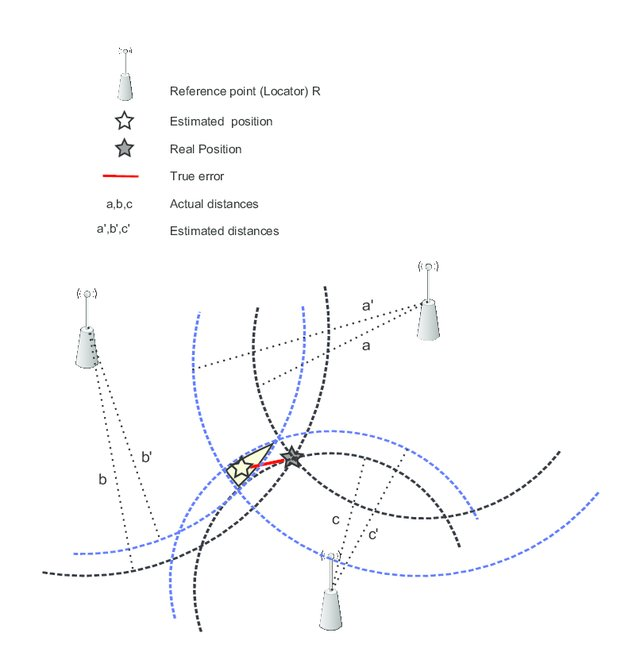
\includegraphics[scale=1]{./images/toa}
            \caption{Técnica de Tiempo de Llegada (ToA)}
            \label{fig:ToA}
        \end{figure}
            
        En ésta técnica, dado que los errores de estimación de distancia se derivan de mediciones de tiempo de salida y llegada del mensaje, se debe procurar que los tiempos sean bien medidos, esto es, que todos los dispositivos transmisor y receptor estén sincronizados en el mismo tiempo. La correcta implementación de un sistema de medición basado en ToA permite filtrar los efectos de la multitrayectoria.\\}
        
        \item {\textbf{\ac{TDoA}}: Esta técnica, acorde a lo mencionado en \cite{17}, cosiste en medir la diferencia de tiempo de llegada de la señal que se envia desde un objeto y que es recibida por otros tres dispositivos.\\
        
        Con TDoA, se puede iniciar la transmisión de la señal en un tiempo desconocido en tanto sea conocido por los otros nodos receptores. Lo único que se requiere para que esto funcione, es que entre los receptores, exista una sincronización de tiempo. Esta técnica, también conocida como Multilateración tiene como obstáculo el hecho de requerir una cantidad significativa de ancho de banda, así como también, el alto costo del equipamiento utilizado para aplicarlo.\\
        
        Y es que la banda usada para la implementación de esta tecnología es la \ac{UWB}, definido por la \ac{FCC} como la porción del espectro electromagnético con frecuencias que van desde los 3.1 hasta los 10.6 GHz.
        
            \begin{figure}[h!]
                \centering
                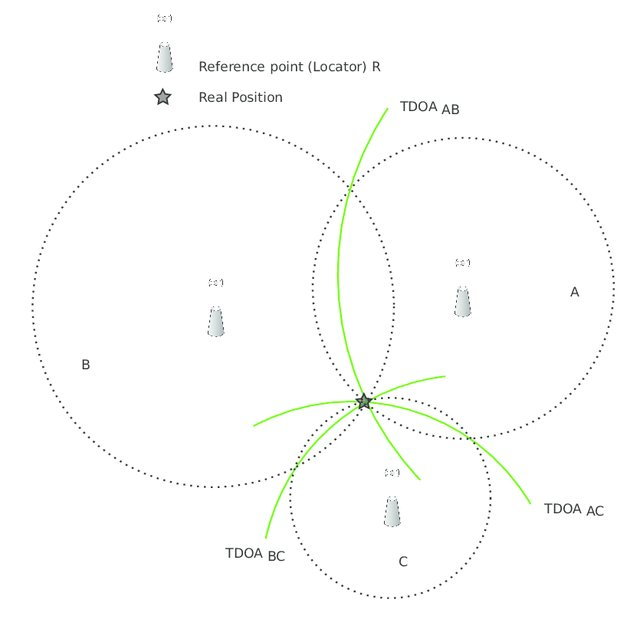
\includegraphics[scale=1]{./images/tdoa}
                \caption{Técnica de Diferencia de Tiempo de Llegada (TDoA)}
                \label{fig:TDoA}
            \end{figure}
        
        }
        \newpage 
        \item {\textbf{\ac{RToF}}: en este método basado en \ref{ToA} que consiste en el tiempo total que toma la conexión entre los dos dispositivos que participan en la comunicación. A diferencia de \ref{fig:TDoA}, acá se considera el tiempo de ida y regreso de la señal, no sólo el tiempo que tarda desde el transmisor hasta el receptor. Este método de medida no requiere ninguna sincronización entre los dispositivos, de modo que se puede implementar necesitan únicamente enviar el resultado de la medición del \ac{RTT} para hacer el cálculo bajo la siguiente fórmula:\\
        
        \begin{equation}
            d = \dfrac{c\cdot{\left(T_{Total} - T_{proc}\right)}}{2}
        \end{equation}
        
        Donde \textit{d}, representa la distancia entre los dos dispositivos; \textit{c}, la velocidad de la luz; Tproc, el tiempo que le toma a la estación realizar el calculo. Siendo este último, un parámetro complejo de obtener con precisión, ya que depende de la latencia del sistema. Esto se escala como la principal desventaja de este sistema ya que calcular la posición para varios dispositivos se traduce en lidiar con latencias que impidan obtener la posición de dispositivos que se mueven rápidamente.
        
        \begin{figure}[h!]
            \centering
            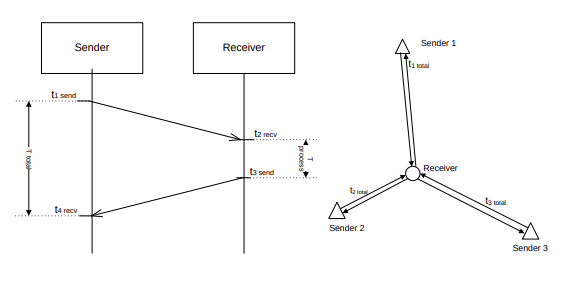
\includegraphics[scale=0.52]{Tesis/images/rtof}
            \caption{Diagrama de medición de distancia usando \ac{RToF}}
            \label{fig:RTOF}
        \end{figure}
        }
    \end{enumerate}
            }

    \item{\textbf{Técnicas basadas en los niveles de intensidad de señal recibida}
    \begin{enumerate}
        \item{\textbf{\ac{RSSI}}: Respecto de esta técnica se tiene que algunos autores la introducen como una técnica propia de algoritmos de Detección de Proximidad (\ref{Detección de Proximidad}}) debido a que los niveles de los indicadores de intensidad de señal recibida, al guardar relación con la distancia, tal y como señalan los modelos de propagación para interiores, establecen que a menor distancia del AP, mayor debe ser la intensidad de señal recibida.\\
        
        Los mismos autores que la clasifican dentro de la sección mencionada, utilizan esta técnica para trazar un sistema de coordenadas basadas en las intensidades recibidas respecto de cada AP, esto les permite mapear la zona en una etapa que llaman offline y ubicar al dispositivo en la etapa posterior, llamada online.\\
            
        En esta etapa, se asigna a través de un sistema de coordenadas, los niveles de intensidad de señal, tal que es posible posicionar el objetivo según los RSS de los AP, como se ve en la imagen.
            
        \begin{figure}[h!]
            \centering
            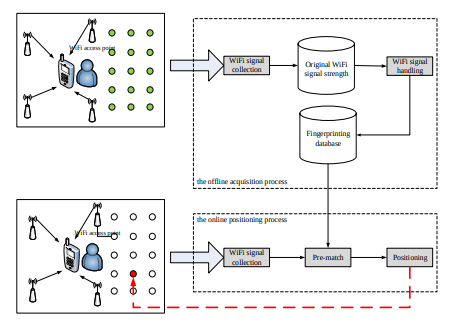
\includegraphics[scale = 0.6]{./images/rssi}
            \caption{Idea de algoritmo basado en RSSI}
            \label{fig:RSSI}
        \end{figure}
        
        \item{Algoritmos de posicionamiento para método por características de posición}\\
        
            \begin{enumerate}
                \item {\textbf{Método Probabilístico}: En este método, se considera el estimar la posición del ibjetivo, como un problema de clasificación, ya que desde un vector de RSS capturadas desde los APs, se puede estimar la probabilidad de que un valor \textit{S}, pertenezca a un AP particular, y por ende, a un punto de coordenadas aproximado. \\
                
                Se puede hacer el cálculo de la posición a través de modelos de inferencia y asociarlo también a un tipo de Cadenas de Markov, así como también, apoyar el cálculo introduciendo medidas de dispersión tales como la desviación estándar y la varianza, o de una medida de tendencia central como es la media.\\
                }
                
%%%%%%%%%%%%%%%%%%%%%%%%%%%%%%%%%%%%%%%%%%%%%%%%%%%%%%%%%%
                \clearpage 
%%%%%%%%%%%%%%%%%%%%%%%%%%%%%%%%%%%%%%%%%%%%%%%%%%%%%%%%%%
                
                \item{\textbf{Método \ac{SVM}}: \label{SVM} En la literatura consultada \cite{7} los autores señalan a esta técnica como \textit{''Una nueva u prometedora técnica para clasificación de datos y Machine Learning.''}, que ha sido usada con resultados satisfactorios en el mapeo de intensidad de señales inalámbricas.\\
                
                Su implementación consiste igualmente en dos fases; una de entrenamiento, que es aquella en que los sets con los datos de  intensidad de señal de los AP son ingresados, y con los cuales se buscará diseñar un hiperplano que clasifique los vectores en dos clases, procurando maximizar la distancia entre estos.\\
                
                \begin{figure}[h!]
                    \centering
                    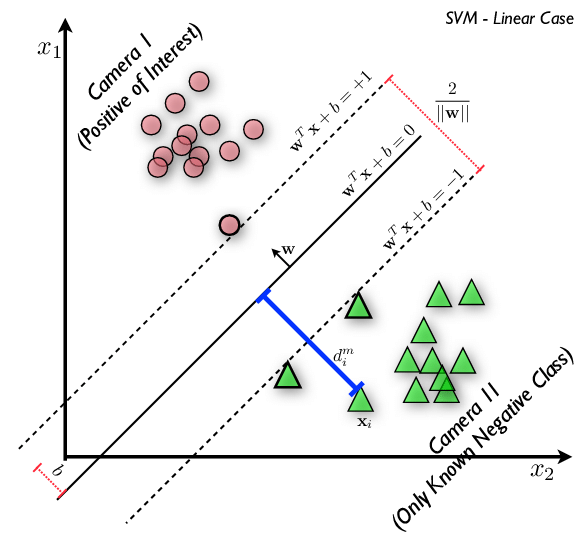
\includegraphics[scale=0.4]{./images/svm}
                    \caption{Distintos hiperplanos para el mismo set de datos.}
                    \label{fig:SVM}
                \end{figure}
                
                Sin embargo, dado que en un espacio indoor, la cantidad de AP es , por lo general, superior a 2, la posibilidad de que en un set de datos podamos diferenciar entre un AP u otro mediante el procedimiento de encontrar el hiperplano que separa maximizando la distancia entre los valores, es nula, e implementar un algoritmo recursivo que vaya evaluando para cada AP, el hiperplano que clasifica la medición del objetivo en alguno de ellos, es costosa computacionalmente además de compleja.\\
                }
%%%%%%%%%%%%%%%%%%%%%%%%%%%%%%%%%%%%%%%%%%%%%%%%%%%%%%%%%%
                \clearpage 
%%%%%%%%%%%%%%%%%%%%%%%%%%%%%%%%%%%%%%%%%%%%%%%%%%%%%%%%%%

                \item {\textbf{Método \ac{KNN}}: El método de vecinos más cercano es uno de los métodos de clasificación más simple dentro de la librería de Machine Learning ya que consiste, en una clasificación por similitud respecto de otros puntos en un dataset de entrenamiento. \\

                El objetivo de este método es el de agrupar vectores de características, que no son más que representaciones matemáticas para la información. Ha de tenerse en cuenta que el vector de características puede requerir un pre procesamiento si es que estas no son necesariamente numéricas, ya que de este modo se podrá agrupar los datos como si se tratara de un vector de $R^{N}$.\\

                Ahora, a diferencia de otros métodos de clasificación, como es el caso de \ref{SVM}, en KNN la fase de entrenamiento no existe, de manera que sólo se trata de una fase. En cambio, se tiene que cualquier caso por abstraer o generalizar la información que allí está, es un hecho en la etapa de clasificación.\\

                Esto significa que se puede trabajar inmediatamente sobre los datos, en tanto estos, tal y como se mencionó previamente, no requieran un pre procesamiento. Dado que lo que hace este método es agrupar valores, el resultado óptimo será cuando exista un reducido número de  data-sets y estos no tengan valores no numéricos.\\

                Así, se tiene que los datos que se clasificarán pueden también ser representados como una matriz de M x N  datos, de donde ; M, es el número de datos; y N, son las características de los datos. Dicho esto, el proceso de agrupamiento de los datos se hace según las siguientes consideraciones:\\

                \begin{itemize}
                    \item {Se calcularán las distancias entre los valores a clasificar, y aquellos contenidos en el data-set. En el cálculo de la distancia suele usarse la distancia euclidiana, que es básicamente, la magnitud del vector que se obtiene al restar un punto de muestra del data-set de entrenamiento, con el punto a clasificar
    
                    \begin{equation}
                        E(x,y) = \sqrt{\sum_{i=0}^{n}({x_{i}-y_{i}})^{2}} \ \ 
                    \end{equation}
                    }

                    \item{Se escogerá un valor \textit{K}, que por lo general, no es ni múltiplo de la cantidad de clases, ni par, y que representa la cantidad de valores \textit{K} con las distancias más bajas. Este puede ser escogido arbitrariamente o bien, en caso que sea necesario, obtenido por validación cruzada. \footnote{La validación cruzada o cross-validation es una técnica utilizada para evaluar los resultados de un análisis estadístico y garantizar que son independientes de la partición entre datos de entrenamiento y prueba.}\\}
                    
                    \item{Finalmente, se agruparán los datos a una clase, a través de la comparación de las distancias obtenidas. Si este, posee la mayoría de los  \textit{K} de puntos cuya distancia los asocia a una clase A, entonces este será clasificado en dicha clase. Si por el contrario, el número de puntos cuya distancia se acerca a los datos objetivo no son mayoría, entonces este pertenecerá a B.\\
                    
                    \begin{figure}[h!]
                        \centering
                        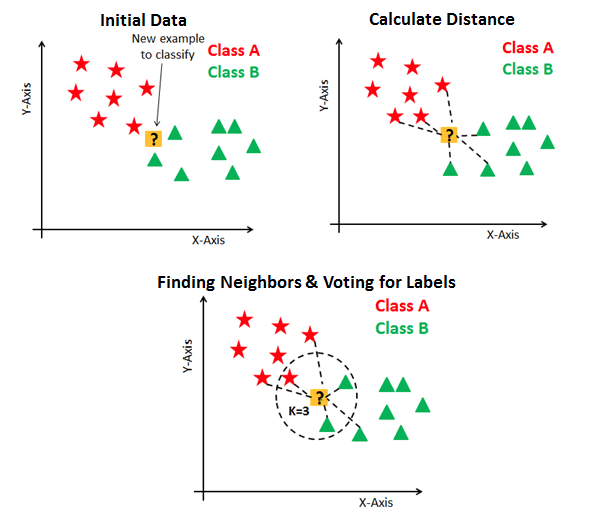
\includegraphics[scale=0.65]{./images/knn}
                        \caption{Representación gráfica del funcionamiento de KNN según el valor de K}
                        \label{fig:KNN}
                    \end{figure}
                    }
            \end{itemize}}
            
            \newpage
            
            \item{\textbf{Método \ac{RNA}}: Este método se vale de una neurona artificial llamada \textbf{perceptrón}, algo que fuera desarrollado entre los años 1950s y 1960s por el científico Frank Rosenblatt, inspirado por el trabajo de Warren McCulloch y Walter Pitts <<A Logical Calculus of the Ideas Immanent in Nervous Activity>> \cite{19} donde señalan la posibilidad de rescatar la idea de un sistema complejo de redes y conexiones, de impulsos y señales, como es nuestro sistema nervioso, y extrapolarlo a uno computarizado, donde en lugar de estímulos, se tuvieran señales.\\
            
             Se mencionó que uno de los objetivos del trabajo de McCulloch fue el de introducir la noción de neurona artificial, por esto es que el perceptrón le debe su estructura, presentada a continuación:
             
            \begin{figure}[h!]
                \centering
                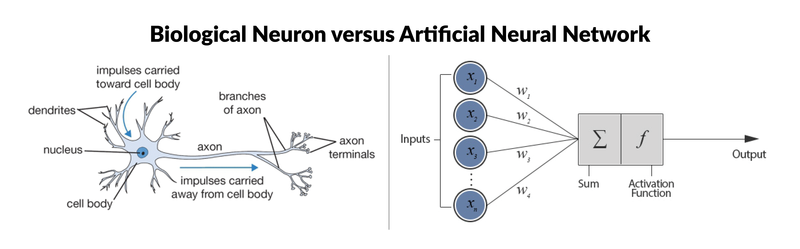
\includegraphics[scale=0.5]{Tesis/images/nn}
                \caption{Comparación por similitud de una neurona con un perceptrón}
                \label{fig:NN}
            \end{figure}
            
            En el cerebro humano, existen distintos tipos de neuronas las cuales están destinadas para tareas específicas, por esta razón, puede darse que una neurona reciba señales de temperatura, presión, luz, entre otras, antes de transmitir un impulso. Este último viene en algunos casos a ser la suma ponderada de los distintos estímulos nerviosos que provienen de las otras terminaciones sinápticas, tal que es en el soma donde se evalúa si esta excede el potencial de acción o no. Si lo hace, la señal será enviada a través del soma y las terminaciones sinápticas hasta un órgano diana u otra neurona, pudiendo ser esta señal inhibitoria, excitadora o moduladora.\\
            
            \begin{figure}
                \centering
                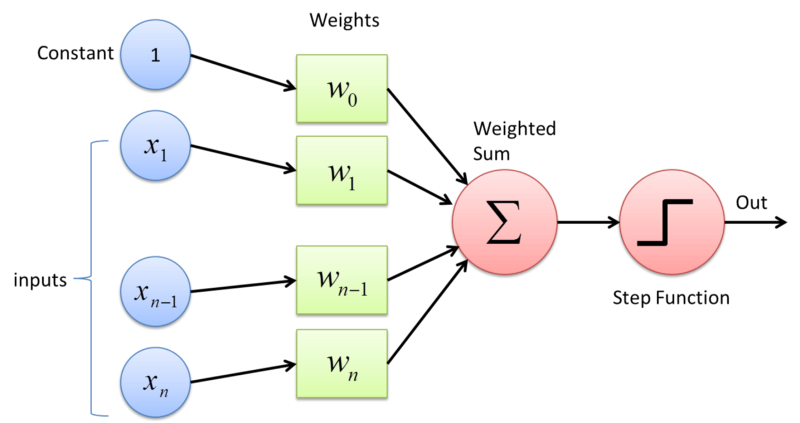
\includegraphics[scale=0.35]{Tesis/images/perceptron}
                \caption{Representación de un Perceptrón}
                \label{fig:Perceptron}
            \end{figure}
            
            Tal como se puede ver en \ref{fig:Perceptron}, se tiene que están las conexiones de la capa de entrada, representadas por impulsos o señales de entrada \textbf{$x_j$}, que luego se multiplican por los pesos \textit{$w_j$} y pasan a evaluarse en la función de activación.\\
            
            Las neuronas son representadas como unidades individuales de procesamiento, que al agruparse forman una red neuronal cuya función de activación, y luego, las capas se resumen en tres:\\
            
            \begin{itemize}
                \item {\textbf{Capa de entrada}: las unidades que componen esta capa son los campos de entrada, por donde ingresan los primeros estímulos}
                
                \item{\textbf{Conexiones ponderadas}: Las operaciones que se realizan en las capas, se logran a través de las fuerzas de conexión variables, o ponderaciones, que resultan del producto entre los pesos \textbf{$w_j$}, que representan la fuerza que tiene un nodo en particular, y los estímulos \textbf{$x_j$}. Los datos de entrada se presentan en la primera capa y estos se propagan a través de las capas ocultas, en forma de \textit{función de propagación},tal cual hiciera el impulso eléctrico en las neuronas, hasta llegar a la capa de salida que es donde el dato de salida, nos permitirá tomar decisiones o evaluar resultados.}
                
                \item{\textbf{Capas Ocultas}:  Son aquellas unidades de procesamiento que transforman el impulso de entrada en otro diferente pero que no son realmente ni una entrada ni una salida.}
                
                \item{\textbf{Función de activación}: Es quizás la característica principal o definitoria de las neuronas, la que mejor define el comportamiento de la misma. Se usan diferentes tipos de funciones, desde simples funciones simples de umbral a funciones no lineales. Se encarga de calcular el nivel o estado de activación de la neurona en función de la entrada total.\\
                
                La función de activación, en este caso Sigmoide, corresponde una función continua no lineal cuyo rango va entre 0 y 1 que puede ser representada gráficamente a través de \ref{fig:sigmoid} y matemáticamente a través de \ref{sigmoid_eq}:\\
            
                \begin{figure}[h!]
                    \centering
                    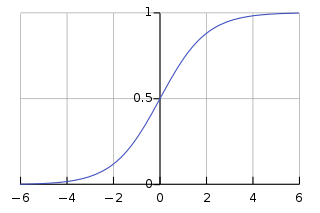
\includegraphics[scale=0.6]{./images/sigmoid}
                    \caption{Función Continua no lineal Sigmoide}
                    \label{fig:sigmoid}
                \end{figure}
            
                \begin{equation}
                    S(u_j) = \dfrac{1}{1+e^{-u_j}}
                    \label{sigmoid_eq}
                \end{equation}
                }       
                
                \item{\textbf{Capa de salida}: Compuesta por una o varias unidades que representan los campos de salida y que entregan el resultado que finalmente es modelado por la siguiente expresión:
                
                \begin{equation}
                    O_j  = S({w_j}{x_j} + {w_0})
                    \label{prob_pred}
                \end{equation}
                
                Donde $w_0$, es el  Bias, una constante que ayuda al modelo de una manera que puede ajustarse mejor a los datos dados y $O_j$, el resultado particular de la evaluación de un dato en la función Sigmoide.\\
                }
            \end{itemize}
            
            Al igual que hace el cerebro por acción de las neuronas, una red es capaz de aprender examinando los registros individuales, generando una predicción para cada uno de estos y ajustando, a través de los pesos, las ponderaciones en caso que el resultado no haya sido el óptimo. Este proceso es iterativo y puede tener lugar cientos de veces antes que la red sea capaz de mejorar sus predicciones antes de alcanzar resultados que satisfagan los criterios de parada.\\
            
            En un comienzo, las ponderaciones son aleatorias, y las respuestas suelen ser muy dispares, sin embargo, y conforme va avanzando el entrenamiento, esta va mejorando, haciéndose más precisa en predecir o replicar a partir de los resultados conocidos.\\
            
            Un aspecto importante, es que a la propagación de las respuestas desde las capas de entrada hacia la capa de salida, se le llama \textit{forward propagation} o \textit{propagación hacia adelante} y cuyo objetivo, así como el del entrenamiento en general es minimizar el costo computacional de la red. Ahora, así como existe la propagación hacia adelante, existe también una hacia atrás llamada \textit{back propagation}, que consiste en reingresar al sistema, la salida resultante de proceso anterior, a fin de optimizar el resultado de los pesos y sesgos. }
            \end{enumerate}
        \end{enumerate}
            }
    \end{itemize}
    
	\chapter{Diseño de algoritmo}
\section{Introducción}
En este capítulo se pretende abordar el diseño para llevar a cabo el objetivo principal y algunos de los específicos del proyecto.

\section{Diseño general de trabajo}
En la figura \ref{fig:esquema} se observan las partes que componen el trabajo del sistema. En este sentido, es necesario hacer una diferenciación entre la parte \textit{offline} y la parte \textit{online} ya que cada parte por separado conlleva requerimientos específicos.

\begin{figure}[h!]
    \centering
    \begin{subfigure}[b]{0.7\textwidth}
        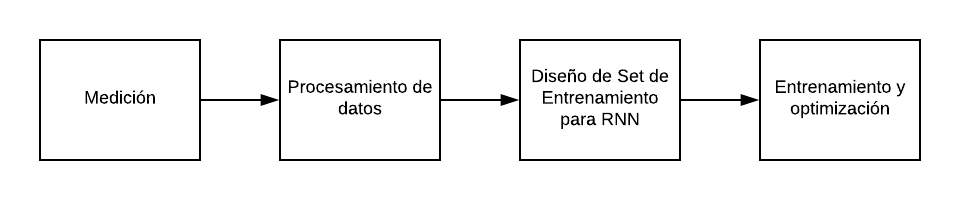
\includegraphics[width=\textwidth]{./images/online}
        \caption{Etapa Online}
        \label{fig:Online}
    \end{subfigure}
    
    \begin{subfigure}[b]{0.4\textwidth}
        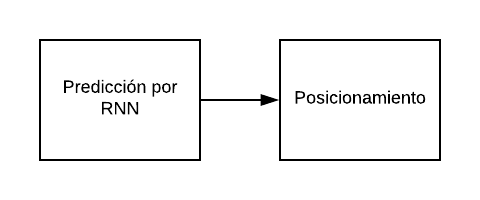
\includegraphics[width=\textwidth]{./images/offline}
        \caption{Etapa Offline}
        \label{fig:offline}
    \end{subfigure}
    \caption{Diagrama General de operación de Algoritmo de posicionamiento}
    \label{fig:esquema}
\end{figure}

\subsection{Offline}
\subsubsection{Medición}

En éste módulo se extraerán los datos usando como hardware, un ordenador de placa reducida como es Raspberry Pi 2 y un Adaptador USB Nano Inalámbrico N de 150Mbps, modelo TL-WN725N. Los cuales tendrán por función medir los niveles de intensidad de potencia de cada uno de los Access Points que se hallen a su alrededor.

% A través del comando \texttt{iwlist}, parte del paquete de herramientas de \texttt{wireless-tools} se recolectarán los niveles de intensidad de señal, las MAC de los AP, así como también del \ac{ESSID} de las redes.

% Para la medición, se dividirá el laboratorio tal que quede como una matriz de 3x3, 3 sectores a lo ancho y 3 a lo largo.

\subsubsection{Extracción y procesamiento de datos}

Para este módulo se trabajará con un algoritmo diseñado cuya función es hacer el pre-procesamiento de los datos. Esto se traduce en que el algoritmo escribe todos la información recopilada en un archivo que posteriormente es leído para filtrar de este sólo los datos que requerimos, esto es; la MAC del AP, el \ac{ESSID}, así como el \ac{RSSI}. Luego, el archivo obtenido corresponde al dataset de entrenamiento que será el usado entrenar la red.

\subsubsection{Diseño de Set de Entrenamiento}

Con el objetivo de relacionar los Niveles de Intensidad de Señal Recibida, con una posición en particular, es menester asociar estos a coordenadas en el espacio, para ello en este punto se leerá el archivo obtenido en puntos anteriores y coordenadas presentadas como pares ordenados, serán incorporados como un elemento más al dataset de entrenamiento.

\subsubsection{Entrenamiento y Optimización}

Dado que en principio, la red es incapaz de percibir la relación existente entre la posición y la densidad de potencia radiada, es preciso relacionar los datos con que se alimenta la red. Por esta razón es necesario hacer un ajuste adicional sobre estos.

Para que el sistema aprenda, es preciso que el dataset sea tan robusto como se pueda. Sin embargo, en lo que respecta a redes neuronales conceptos como  sobreajuste(\textit{\glsenablehyper\gls{Overfitting}}) y  subajuste(\textit{\glsenablehyper\gls{Underfitting}}) llevan a poner especial cuidado en que el sistema, con un número óptimo de iteraciones, datos y neuronas, funciones de activación y capas, alcance efectivamente el resultado deseado.

Por ello se implementarán técnicas de optimización de redes neuronales que cuidarán que los parámetros antes mencionados no lleven a resultados que sean distintos de los óptimos.

\subsection{Online}

\subsubsection{ANN para estimar la posición del objetivo.}

En este punto, se tomarán nuevas muestras de intensidad de señal a fin de entregarlas valores de prueba para predecir, según lo que aprendió la red en su entrenamiento, cuaĺ es la posición en que se haya el objetivo.

Como salida de la red se tendrá la posición y la precisión con que esta fue estimada.
	\chapter{Implementación}
\section{Introducción}

En este capítulo se describirá la implementación del proyecto, dando énfasis en las tecnologías y dispositivos usados para el posicionamiento.

\section{Implementación general de trabajo}
A continuación, se observa el esquema general del algoritmo a implementar y cómo confluyen ambas partes para llevar a cabo el posicionamiento.

\begin{figure}[h!]
    \centering
    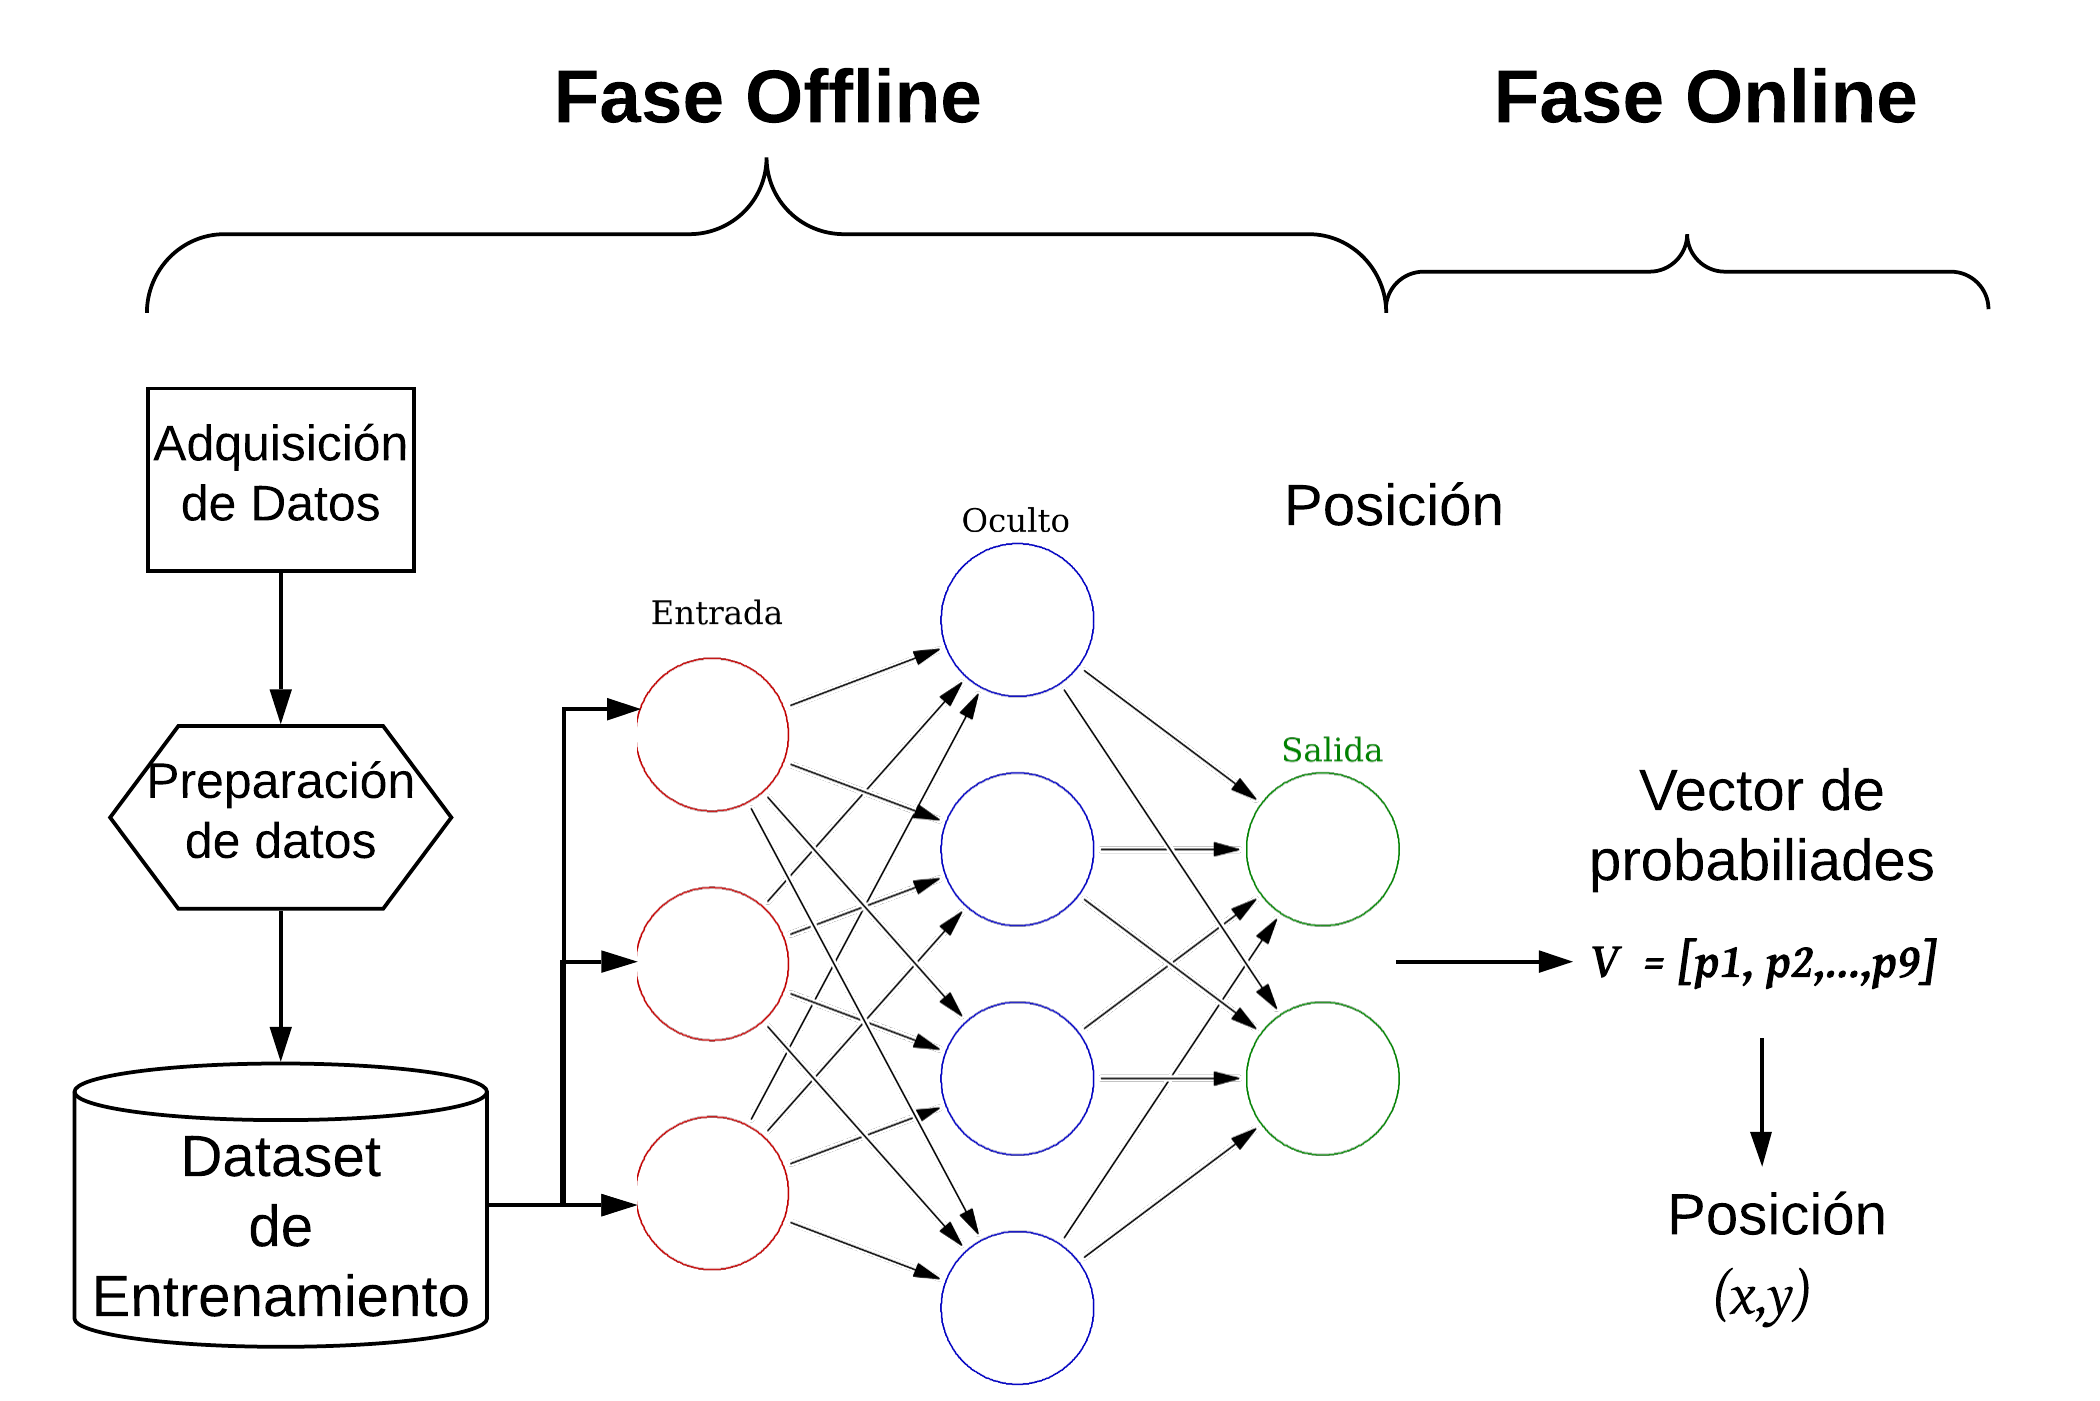
\includegraphics[scale=0.15]{./images/esquema2}
    \caption{Esquema de Implementación General de Trabajo}
    \label{fig:esquema2}
\end{figure}


\subsection{Fase Offline}
\subsubsection{Adquisición de RSSI}
La adquisición de estos datos se hará con la librería de linux llamada \texttt{iwlist}. Una breve descripción de esta, a continuación:

\begin{itemize}
    \item{\textbf{Descripción}: Iwlist es usada para mostrar información adicional de dispositivos inalámbricos de una red. El argumento principal es usado para seleccionar una categoría de información, \texttt{iwlist} muestra información en detalle para toda la información relacionada a esta categoría, incluyendo la información que se muestra en \texttt{iwconfig}.}
    
    \item {\texttt{Scan}: Entrega una lista completa de los Access Points y celdas Ad-Hoc en el rango, y opcionalmente, información adicional sobre ellos. Algunos de estos datos adicionales son \texttt{ESSID, Quality, Frequency, Mode, etc} que permiten entre otras cosas, reconocer la \textbf{dirección MAC} de los dispositivos, el \textbf{RSSI}, y el \textbf{nombre de la red}.
    
    \begin{figure}[h!]
        \centering
        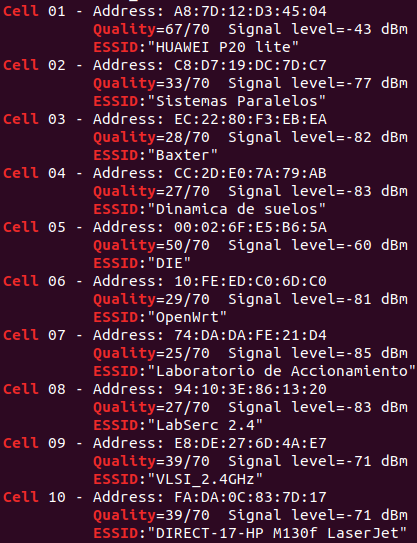
\includegraphics[scale=0.5]{./images/output}
        \caption{Salida de consola con datos de AP}
        \label{fig:output}
    \end{figure}
    
    En esta parte, es necesario recalcar que las características a desplegar dependerán de la tarjeta de red de manera que para efectos del proyecto, se limitarán al adaptador de red inalámbrico conectado a la raspberry pi}
\end{itemize}

Con lo mencionado anteriormente podemos hacer un mapeo del laboratorio tal que para una posición específica sea, por ejemplo $(x,y) = (0,0)$ el punto de origen de las mediciones, puedan obtenerse los niveles de intensidad de señal. De este modo, extendiendo esta metodología a las demás posiciones es que se caracterizará el espacio en función del parámetro RSSI en \ref{fig:esquema}.

Las mediciones se harán en espacio accesible y de trafico relativamente bajo como es el laboratorio de redes de datos. Este para efectos prácticos fue dividido en dos partes como se presenta en la siguiente imagen:

\begin{figure}[h!]
    \centering
    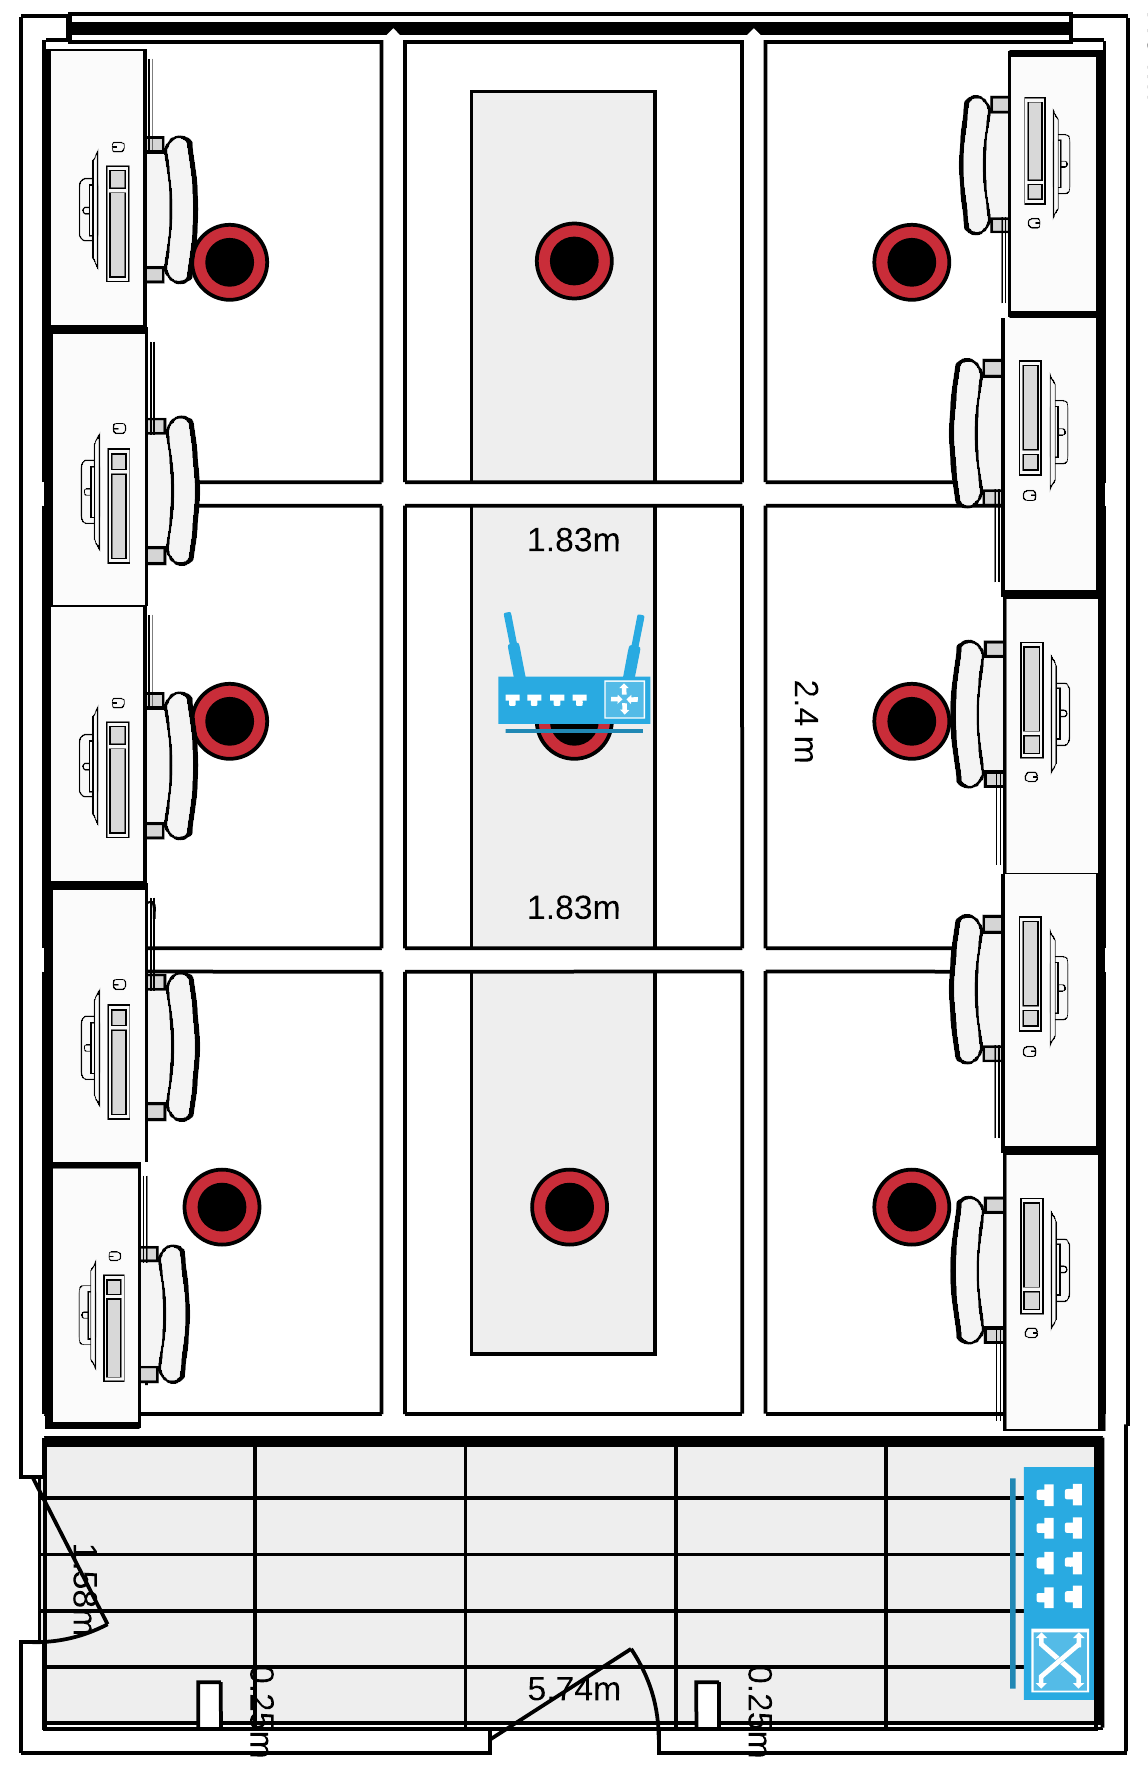
\includegraphics[angle=90,origin=c,scale=0.2]{./images/maplab}
    \caption{Mapa Lab. de Redes de datos}
    \label{fig:mapalab}
\end{figure}

\begin{itemize}
    \item {\textbf{Escritorios y computadores}: corresponden a la parte que no está ennegrecida y que fue dividida en 9 sectores de 2.4 x 1.83 m en los cuales se dispusieron los equipos -representados a través de los puntos rojos con negro, a una altura de 0.8 m para así medir. Estos fueron ubicados equidistantes uno de otro.}
    \item{\textbf{Franja no utilizable}: este sector corresponde a un espacio que dada su relación asimétrica de profundidad y densidad de materiales no fue considerado en el estudio.}
\end{itemize}

\subsubsection{Set de entrenamiento}
En esta parte, los datos son filtrados, separados y agrupados en un archivo \texttt{.csv} para la posterior lectura y procesamiento de la Red Neuronal.

El formato de los datos de entrada proveídos a la red es el siguiente.
\begin{figure}[h!]
    \centering
    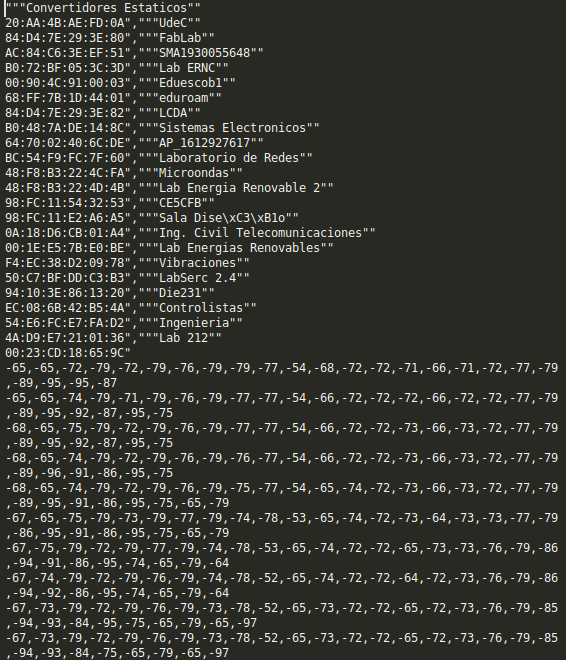
\includegraphics[scale=0.5]{./images/plaincsv}
    \caption{Formato tipo de datos entregados }
    \label{fig:datos}
\end{figure}

Del listado anterior cabe recalcar que lo único relevante es la potencia recibida, medida en dBm, desde los AP cercanos. La información de las etiquetas de las columnas resulta prescindible por cuanto no es objeto de interés de este trabajo, el establecer una correlación entre los RSSI de AP específicos y la posición de un objetivo, sino el hacerlo indistintamente de cuál sea el AP.

\newpage

\subsection{Red Neuronal}

La red neuronal se compone de las siguientes capas:

\begin{itemize}
    \item \textbf{Capa de entrada}: Esta capa recibirá tantos valores de entrada como mediciones de RSSI haya para el total de posiciones que se desee estimar. Esto se traduce en la práctica en obtener el número de filas del archivo \texttt{csv} mencionado previamente.
    
    \item{\textbf{Capas ocultas o \textit{Hidden layers}}: Corresponde al espacio intermedio existente entre la capa de entrada y la capa de salida, que bien puede tratarse de una o varias capas que propagan los valores de entrada hacia la salida ajustando según sea necesario, los pesos que llevan, en este caso, lo valores de RSSI a una predicción correcta.}
    
    \item{\textbf{Capa de salida:} Corresponde a la capa final del modelo y representa la salida de la red. En este caso, sus valores de salida son la probabilidad con que se estima que pueda ser cada posición. De este modo, para un valor de entrada, es decir, un vector de potencias, la salida luego del paso de la red corresponde a una lista con las probabilidades de que sea una u otra posición. Cabe mencionar que posterior a la salida, debe ejecutarse una interpretación de los resultados, esto es, traducir desde lo que son las probabilidades, a lo que es una posición dada.}
\end{itemize}

\begin{figure}[h!]
    \centering
    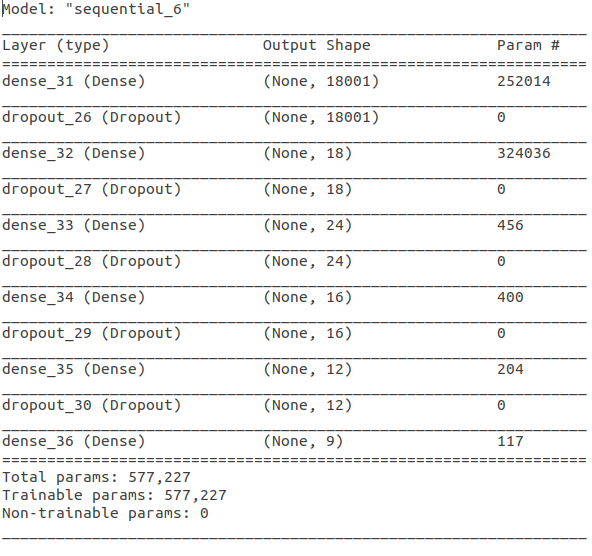
\includegraphics[scale=0.4]{./images/summary}
    \caption{Diagrama de funcionamiento offline}
    \label{fig:Red_offline}
\end{figure}

% \textbf{La red será implementada usando la biblioteca de redes neuronales \texttt{Keras}, la cual es biblioteca de Redes Neuronales OpenSource escrita en Python y está diseñada para facilitar la experimentación con redes de Deep Learning. Se caracteriza por ser amigable para el usuario, modular y extensible.}

% Un aspecto sumamente importante a mencionar es que si bien al finalizar el entrenamiento de la red, esta arroja un valor de precisión con que es capaz de predecir un valor de salida según valor de entrada dado, se tiene que este indicador no refleja con seguridad el comportamiento de la red. Es por esto, que nos valdremos de técnicas que arrojan ciertas otras métricas tales como varianza, precisión, exactitud y matriz de confusión, así como también, parámetros que permiten comprender con mayor certidumbre cómo se procesará y predecirá los datos nuestra red.

Es sobre estas capas en las que se aplicarán las técnicas de Cross-validation y Grid-Search para entregar información respecto de; cuál es el valor de las métricas que reflejan el comportamiento real de la red y cuáles son los parámetros (n$^\circ$ de capas y epochs, optimizador y batch-size) y con ello, optimizar el funcionamiento de la red. Cabe mencionar, que dentro de los indicadores que se obtendrán se encuentra la Matriz de Confusión, con esta se apoyará la exactitud y precisión de la red.

	\chapter{Resultados}
\section{Introducción}
\section{Implementación general de trabajo}
\section{Medición}
\section{Extracción}
\section{Visualización}
	\chapter{Conclusiones}

% ***********************************************************************************
\section{Sumario}
Dentro del desarrollo del estudio, se contemplaron diversos enfoques, se ponderó la posiblidad de implementar en la memoria de título un sistema de posicionamiento indoor basándose en algoritmos de estimación de posición geométricos y otros, en parámetros más complejos, no obstante, la poca practicidad y adaptabilidad de estos modelos al ambiente donde se podría implementar, supone una desventaja innegable.

% ***********************************************************************************
\section{Conclusiones}
Por todo lo revisado, estudiado y expuesto, se plantea la posibilidad de que, como alternativa a los algoritmos geométricos o basados en potencia, se consideren alternativas más efectivas, de menor coste computacional y que no dependan de parámetros relacionados con el ambiente, dado que en ambientes indoor o en sectores muy concurridos hay métricas que varían considerablemente, al punto de obligar a realizar mediciones correctivas.

Además, se tiene que la efectividad y precisión del método que recoge las solicitudes IRDP, es considerablemente superior al no depender de otros parámetros salvo la llegada de los paquetes al router.

Se dio cumplimiento a los objetivos planteados inicialmente, mediante la investigación de las alternativas, que fueron abordadas a fondo a través de literatura. Se pudo llegar a una comprensión justificada de las ventajas y desventajas de los métodos, pudiendo así, escoger con base en distintos estudios teóricos y empíricos, cuál es el método que convendría desarrollar en detalle en la memoria de título.

En suma, se destaca la importancia de llegar a desarrollar un sistema de posicionamiento indoor que cuente con una precisión que no sea directamente proporcional a la capacidad de cómputo, tanto si se desea resolver necesidades humanas tales como, hallar la mejor ruta de acceso para una persona con capacidades diferentes, a través de una aplicación móvil que desde el seguimiento de su interfaz vaya dándole instrucciones. Como si se desea implementar un sistema que recoja las solicitudes de los clientes que desean conectarse y con ello, hacer un seguimiento de las posiciones, a fin de que este, permita generar reportes e informes estadísticos que relacionen patrones de conducta y también de consumo, que favorezcan a un mejoramiento en las estrategias de venta y en la experiencia de compra del cliente.

% ***********************************************************************************
\section{Trabajo Futuro}
Se listan las posibles líneas de investigación que se deducen directamente de la presente obra.

\begin{enumerate}
\item {Implementación de un sistema que realice el seguimiento de las solicitudes IRDP donde pueda visualizarse el movimiento de las interfaces de red}
\item{Realizar un estudio que contraste la precisión y eficacia con la que los métodos geométricos y el de las solicitudes IRDP realizan la estimación de posición.}
\item{Estudiar algoritmos de posicionamiento basado en redes neuronales.}
\item{Estudiar la precisión de las mediciones obtenidas por el uso del sistema presentado en \cite{8}}
\end{enumerate}

Se quiere que al menos existan unas 3 a 5 ideas en las que se pueda seguir investigando.
% ***********************************************************************************
%\section{Publicación}
%A veces, los trabajos dan pie a una publicación en conferencia o revista. Es importante mencionarlo en esta sección.


% ******************** Bibliografía ********************
\pdfbookmark{Bibliografía}{bibliografia}
%\chapter{Bibliografía}

\begin{thebibliography}{X}
\bibitem{1} \textsc{Van Vinh Nguyen} y \textsc{Weon Lee Jong}, <<Self-Positioning System for Indoor Navigation on Mobile Phones>> \textit{IEEE International Conference on Consumer Electronics (ICCE), 2012}

\bibitem{2} \textsc{Rea Mauricio, Cordobés Héctor, Gustiniano Domenico},<<Twins: Time-of-flight based Wireless Indor Navigation System>>

\bibitem{3} \textsc{Bianca Bobescu, Marian Alexandru} <<Mobile indoor positioning using Wifi localization>> Review of the Air Force Academy. Transilvania University, Brasov, Romania

\bibitem{4} \textsc{Mayur Tawari},\textsc{Onkar Pathak},\textsc{Rajesh Palaskar} y \textsc{Rajesh Palkar}, <<Wi-Fi Indoor Positioning System Based on RSSI Measurements from Wi-Fi Access Points –A Tri-lateration Approach>>, \textit{International Journal of Scientific \& Engineering Research. V5}, 2014.

\bibitem{5} \textsc{C. Yang and H. r. Shao}, <<WiFi-based indoor positioning,>> in IEEE Communications Magazine, vol. 53, no. 3, pp. 150-157, March 2015. doi: 10.1109/MCOM.2015.7060497

\bibitem{6} \textsc{Zahid Farid, Rosdiadee Nordin} y \textsc{Mahamod Ismail}, <<Recent Advances in Wireless Indoor Localization Techniques and System>>, \textit{Journal of Computer Networks and Communications}, 2013.

\bibitem{7} \textsc{Zhao Kai, Li Binghao} y \textsc{Andrew Dempster}, <<A Comparison of algorithms adopted in fingerprinting indoor positioning systems>>, \textit{IGNSS Symposium}, 2013.

\bibitem{8} \textsc{Ma, R., Guo, Q., Hu, C., \& Xue, J.} (2015). <<An Improved WiFi Indoor Positioning Algorithm by Weighted Fusion>>. Sensors.

\bibitem{9} \textsc{Habibi Lashkari, Arash \& Parhizkar, Behrang \& Ng Ah Ngan, Mike.} (2010). <<WIFI-based indoor positioning system>>. Computer and Network Technology, International Conference on. 76-78. 10.1109/ICCNT.2010.33. 

\bibitem{10} \textsc{Zourmand A., Sheng N., Lai Kun A., et al},<<Human Counting and Indoor Positioning System Using WiFi Technology>> , \textit{IEEE, International Conference on Automatic Control and Intelligent Systems.} October 20,2018, Shah Alam, Malaysia.

\bibitem{11} \textsc{Davies K., Jones I.} y \textsc{Shapiro J.},<<A Bayesian Approach to Dealing with Device Heterogeneity in an Indoor Positining System , \textit{International Conference on Indoor Positioning and Indoor Navigation.} September 2018, Nantes, France.

\bibitem{12} \textsc{Le Dortz N, Zetterberg P. & Gain F.}, <<Wifi Fingerpirnt Indoor Positioning System Using Probability Distribution Comparison>>, \textit{IEEE ICASSP 2012}
\bibitem{13} \textsc{Beom-Ju Shin, Kwang-Won Lee, Sun-Ho Choi, et al},<<Indoor WiFi positining System fior Android Based Smartphone>> , \textit{ICTC 2010}

\bibitem{14} \textsc{Lu Y., Zhang D. Cheng Y., et al},<<An Improved Method and Implementation of Indoor Positioning Fingerprint Matching Localization Based on WLAN>>, \textit{Springer Nature},Switzerland AG 2019

\bibitem{15} \textsc{},<<Towards the Implementation of Recurrent Neural Networks Schemes for WiFi Fingerprint-Based Indoor Positioning>> , \textit{IEEE 2018}

\bibitem{16} \textsc{Y Lu et al},<<Implementation of Fingerprint Matching Method for Indoor Position Based on Virtual Reality Technology>>
\end{thebibliography}

\begin{thebibliography}{X}
\bibitem{1} \textsc{Van Vinh Nguyen} y \textsc{Weon Lee Jong}, <<Self-Positioning System for Indoor Navigation on Mobile Phones>> \textit{IEEE International Conference on Consumer Electronics (ICCE), 2012}

\bibitem{2} \textsc{Rea Mauricio, Cordobés Héctor, Gustiniano Domenico},<<Twins: Time-of-flight based Wireless Indor Navigation System>>

\bibitem{3} \textsc{Bianca Bobescu, Marian Alexandru} <<Mobile indoor positioning using Wifi localization>> Review of the Air Force Academy. Transilvania University, Brasov, Romania

\bibitem{4} \textsc{Mayur Tawari,Onkar Pathak,Rajesh Palaskar \& Rajesh Palkar}, <<Wi-Fi Indoor Positioning System Based on RSSI Measurements from Wi-Fi Access Points –A Tri-lateration Approach>>, \textit{International Journal of Scientific \& Engineering Research. V5}, 2014.

\bibitem{5} \textsc{C. Yang and H. r. Shao}, <<WiFi-based indoor positioning,>> in IEEE Communications Magazine, vol. 53, no. 3, pp. 150-157, March 2015. doi: 10.1109/MCOM.2015.7060497

\bibitem{6} \textsc{Zahid Farid, Rosdiadee Nordin \& Mahamod Ismail}, <<Recent Advances in Wireless Indoor Localization Techniques and System>>, \textit{Journal of Computer Networks and Communications}, 2013.

\bibitem{7} \textsc{Zhao Kai, Li Binghao} y \textsc{Andrew Dempster}, <<A Comparison of algorithms adopted in fingerprinting indoor positioning systems>>, \textit{IGNSS Symposium}, 2013.

\bibitem{8} \textsc{Ma, R., Guo, Q., Hu, C., \& Xue, J.} (2015). <<An Improved WiFi Indoor Positioning Algorithm by Weighted Fusion>>. Sensors.

\bibitem{9} \textsc{Habibi Lashkari, Arash \& Parhizkar, Behrang \& Ng Ah Ngan, Mike.} (2010). <<WIFI-based indoor positioning system>>. Computer and Network Technology, International Conference on. 76-78. 10.1109/ICCNT.2010.33. 

\bibitem{10} \textsc{Zourmand A., Sheng N., Lai Kun A., et al},<<Human Counting and Indoor Positioning System Using WiFi Technology>> , \textit{IEEE, International Conference on Automatic Control and Intelligent Systems.} October 20,2018, Shah Alam, Malaysia.

\bibitem{11} \textsc{Davies K., Jones I.} y \textsc{Shapiro J.},<<A Bayesian Approach to Dealing with Device Heterogeneity in an Indoor Positining System>>, \textit{International Conference on Indoor Positioning and Indoor Navigation.} September 2018, Nantes, France.

\bibitem{12} \textsc{Le Dortz N, Zetterberg P. and Gain F.}, <<Wifi Fingerpirnt Indoor Positioning System Using Probability Distribution Comparison>>, \textit{IEEE ICASSP 2012}

\bibitem{13} \textsc{Beom-Ju Shin, Kwang-Won Lee, Sun-Ho Choi, et al},<<Indoor WiFi positining System fior Android Based Smartphone>> , \textit{ICTC 2010}

\bibitem{14} \textsc{Lu Y., Zhang D. Cheng Y., et al},<<An Improved Method and Implementation of Indoor Positioning Fingerprint Matching Localization Based on WLAN>>, \textit{Springer Nature},Switzerland AG 2019

\bibitem{15}\textsc{H. Hsieh, S. W. Prakosa and J. Leu}, <<Towards the Implementation of Recurrent Neural Network Schemes for WiFi Fingerprint-Based Indoor Positioning,>> 2018 IEEE 88th Vehicular Technology Conference (VTC-Fall), Chicago, IL, USA, 2018, pp. 1-5.doi: 10.1109/VTCFall.2018.8690989

\url{http://ieeexplore.ieee.org/stamp/stamp.jsp?tp=&arnumber=8690989&isnumber=8690547}

\bibitem{16} \textsc{Y Lu et al},<<Implementation of Fingerprint Matching Method for Indoor Position Based on Virtual Reality Technology>>, \textit{An Improved Method and Implementation}

\bibitem{17} \textsc{Alarifi, Abdulrahman \& Al-Salman, AbdulMalik \& Alsaleh, Mansour \& Alnafessah, Ahmad \& Alhadhrami, Suheer \& A. Al-Ammar, Mai \& Al-Khalifa, Hend}. (2016). <<Ultra Wideband Indoor Positioning Technologies: Analysis and Recent Advances>>. Sensors. 16. 1-36. 10.3390/s16050707.

\bibitem{18} \textsc{Lukasz Zwirello, Tom Schipper, Marlene Harter, and Thomas Zwick}, <<UWB Localization System for Indoor Applications: Concept, Realization and Analysis>>, Journal of Electrical and Computer Engineering, vol. 2012, Article ID 849638, 11 pages, 2012. \url{https://doi.org/10.1155/2012/849638.}

\bibitem{19}\textsc{McCulloch, W.S. \& Pitts, W.} <<A logical calculus of the ideas immanent in nervous activity>> Bulletin of Mathematical Biophysics (1943) 5: 115. 

\url{https://doi.org/10.1007/BF02478259}

\bibitem{20} \textsc{K. E. Jeon, J. She, P. Soonsawad and P. C. Ng}, <<BLE Beacons for Internet of Things Applications: Survey, Challenges, and Opportunities>> in IEEE Internet of Things Journal, vol. 5, no. 2, pp. 811-828, April 2018. doi: 10.1109/JIOT.2017.2788449
\url{http://ieeexplore.ieee.org/stamp/stamp.jsp?tp=&arnumber=8242361&isnumber=8334665}

\bibitem{21} \textsc{R. P and M. L. Sichitiu}, <<Angle of Arrival Localization for Wireless Sensor Networks,>> 2006 3rd Annual IEEE Communications Society on Sensor and Ad Hoc Communications and Networks, Reston, VA, 2006, pp. 374-382. doi: 10.1109/SAHCN.2006.288442

\url{http://ieeexplore.ieee.org/stamp/stamp.jsp?tp=&arnumber=4068140&isnumber=4068087}

\bibitem{22} \textsc{Luo, Juan \& Yin, Xixi \& Zheng, Yanliu \& Wang, Chunhua.} (2018). <<Secure Indoor Localization Based on Extracting Trusted Fingerprint>>. Sensors. 18. 469. 10.3390/s18020469.

\bibitem{23} \textsc{Zhou, J \& Li, W \& Jin, L \& Chen, X.} (2015). <<Indoor positioning system based on KNN-SVM algorithm.>> 43. 517-520. 10.13245/j.hust.15S1123.

\bibitem{24}\textsc{Dari, Yohanes \& Suyoto, Suyoto \& Pranowo, Pranowo.} (2018). CAPTURE: <<A Mobile Based Indoor Positioning System using Wireless Indoor Positioning System.>> International Journal of Interactive Mobile Technologies (iJIM). 12. 61. 10.3991/ijim.v12i1.7632. 

\bibitem{25} \textsc{Ren, Jin \& Yunan, Wang \& Changliu, Niu \& Wei, Song}. (2019). <<A Novel High Precision and Low Consumption Indoor Positioning Algorithm for Internet of Things.>> IEEE Access. PP. 1-1. 10.1109/ACCESS.2019.2924992.

\bibitem{26}\textsc{Chen, Chih-Yung \& Yin, Li-Peng \& Chen, Yu-Ju \& Hwang, Rey-Chue}. (2012). <<A modified probability neural network indoor positioning technique>>. Proceedings - 3rd International Conference on Information Security and Intelligent Control, ISIC 2012. 317-320. 10.1109/ISIC.2012.6449770.

\bibitem{27} \textsc{Mu, Zhou \& Yubin, Xu \& Lin, Ma}. (2009).<<ANN indoor position determination based on area correlation in WLAN environment.>> 2009 International Conference on Wireless Communications and Signal Processing, WCSP 2009. 10.1109/WCSP.2009.5371722. 

\bibitem{28} \textsc{F Malik, R \& Gustifa, R \& Farissi, A \& Stiawan, Deris \& Ubaya, H \& Ahmad, Mohd Riduan \& Al-Khaleefa, Ahmed. (2019)}.<<The Indoor Positioning System Using Fingerprint Method Based Deep Neural Network.>> IOP Conference Series: Earth and Environmental Science. 248. 012077. 10.1088/1755-1315/248/1/012077. 

\bibitem{29} \textsc{Antonio Gulli \& Sujit Pal}
<<Deep Learning with Keras>> Birmingham, England : Packt Publishing, 2017. 
\end{thebibliography}


% ******************** Anexos ********************
	\appendix
%	\chapter{Códigos}

%*******************************************************************************%
\section{Derivación de fórmulas}

Lorem ipsum dolor sit amet, consectetur adipiscing elit, sed do eiusmod tempor incididunt ut labore et dolore magna aliqua. Ut enim ad minim veniam, quis nostrud exercitation ullamco laboris nisi ut aliquip ex ea commodo consequat.


%*******************************************************************************%
\section{Unidades especiales}

Lorem ipsum dolor sit amet, consectetur adipiscing elit, sed do eiusmod tempor incididunt ut labore et dolore magna aliqua. Ut enim ad minim veniam, quis nostrud exercitation ullamco laboris nisi ut aliquip ex ea commodo consequat.

	
\end{document}